% this file is called up by thesis.tex
% content in this file will be fed into the main document

%: ----------------------- introduction file header -----------------------
\chapter{Introduction}\label{chapter:intro}

\graphicspath{{X/figures/EPS/}{1_introduction/figures/}}

%ABSTRACT-----------------------------------------------------
\hrule height 1mm
\vspace{0.5mm}
\hrule height 0.4mm 
\noindent 
\\ {\it 
An overview of the properties of sunspot groups, solar activity, and the global magnetic field of the Sun is given in this chapter. The structure of the Sun is described, from the core to the outer atmosphere. The birth, evolution, and decay of sunspot groups and their connection to the large-scale magnetic field over the solar cycle is explained. Then, the properties of active sunspot  groups and the eruptions they produce are discussed. Finally, the aims of this thesis are summarised.
}
\\ 
\hrule height 0.4mm
\vspace{0.5mm}
\hrule height 1mm 
\vspace{1.5cm}
%\newpage
%END ABS---------------------------------------------------------

% ----------------------------------------------------------------------
%: ----------------------- introduction content ----------------------- 
% ----------------------------------------------------------------------

Carl Sagan maintains, ``the Sun is an ordinary, even a mediocre star" \citep{Sagan:1980}. While this statement makes our nearest star sound both mundane and uninteresting, the Sun provides a unique perspective on the physics of the average star. Unlike other stars that are effectively point sources, the Sun can be studied with unparalleled spatial resolution with a telescope. This permits us to spatially resolve features covering a small fraction of the solar disk, such as sunspots, magnetic loops, and coronal holes. The internal mechanics of the Sun may be inferred from studies of these features. For example, the solar activity cycle was discovered due to long-term observations of sunspots. Long-term photometric observations show that certain distant stars exhibit a cyclic variability \citep{Metcalfe:2010}; studies of the Sun indicate the phenomenon is tied to a magnetic dynamo \citep{Parker:1955}. The physics of distant, spatially unresolved solar-type stars can thus be understood from detailed studies of our closest stellar neighbor. 

The following sections provide a general discussion of the Sun as a star as well as our observational and theoretical knowledge of its long- and short-term dynamics. The current state of knowledge regarding the phenomena studied in this work is discussed. This includes the 22-year magnetic cycle, the 11-year activity cycle, the evolution of sunspot groups, and the large-scale transport of magnetic fields dispersing from decaying sunspot groups.


%%%%%%%%%%%%%%%%%%%%%%%%%%%%%%%%%%%%%%%%%%%%
\section{The Sun as a Star}
%%%%%%%%%%%%%%%%%%%%%%%%%%%%%%%%%%%%%%%%%%%%

The Sun is the nearest star to the Earth. Its existence is the result of the collapse of a cloud of interstellar gas and dust which initially reached an equilibrium between the inward force of gravitation and outward pressure forces, including that due to the subsequent energy release from nuclear fusion. The Sun is a Population I star, indicating that it may have emerged from the remains of two preceding generations of stars (Populations II and III). The ejected gas due to the energetic deaths of giant stars (supernovae) from early stellar populations contains heavy elements, fused from lighter elements during the explosions. The Sun later accreted this gas as it formed in the interstellar medium. The Sun has a mainly cosmic composition: 73.46\% hydrogen, 24.85\% helium, and 1.69\% heavier elements, by mass. 

In the standard stellar model, hydrostatic equilibrium is assumed throughout the solar interior. The force of gravity compresses material radially inward, resulting in an opposing force due to the resulting gradient in gas pressure,
\begin{equation}\label{eqn:hydroeq}
\frac{dP}{dr} = -G\frac{M_r\rho}{r^2} \mbox{\,,}
\end{equation}
where $M_r$ is the mass contained within a given radius and $G$ is the gravitational constant. The pressure ($P$), density ($\rho$), and temperature ($T$) decrease monotonically with radius ($r$) from the centre to the solar surface. The majority of stars undergoing fusion are governed by the same force balance between gas pressure and gravity\footnote{radiation pressure is negligible in the Sun, but plays a dominant role in the largest stars. Also, electron and neutron degeneracy  pressures support white dwarf and neutron star interiors, respectively}. The gas pressure is helped by radiation originating from fusion in the core, contributing to internal heating as well as a radiative pressure force.

%\begin{figure}[!t]
%\centerline{\includegraphics[width = 0.9\textwidth]{bbcurvesun.eps}}
%\caption[A comparison between the theoretical and observed flux.]{A comparison between the theoretical and observed spectral irradiance (Equation \ref{eqn:bbspec}) at 1\,AU, assuming the Sun is a black-body. The solar spectrum is a composite of data from several spectral irradiance instruments during the Whole Heliosphere Interval (see: \url{http://lasp.colorado.edu/lisird/}).}\label{fig:blackbodydata}
%\end{figure}

\begin{figure}[!t]
\centerline{\includegraphics[width = 0.9\textwidth]{black_body_aschw.eps}}
\caption[A comparison between the theoretical and observed solar flux.]{A comparison between the theoretical and observed solar flux over wavelength. The thick line shows the observed solar spectrum with emission and absorption lines at short and long wavelengths, respectively. A 5\,762\,K black body spectrum is indicated by the thin line \citep[from][]{Aschwanden:2005}.}\label{fig:blackbodydata}
\end{figure}

It is also assumed that \gls{LTE} is reached, implying that stellar material is thermalised and that both the material and radiation field are in equilibrium. The material is assumed to radiate as a black-body (perfect efficiency of absorption and emission). In \gls{LTE} the distance particles travel between collisions is much smaller than the length-scale over which temperature varies, the temperature scale height, $T/(dT/dr)$. The Planck function gives the distribution of energy emitted as a function of temperature and wavelength,
\begin{equation}\label{eqn:bbspec}
B_\lambda(T)=\frac{2hc^2/\lambda^5}{e^{hc/\lambda k_B T}-1} \mbox{\,,} 
\end{equation} 
which has units of erg\,s$^{-1}$\,cm$^{-2}$. Here, $h$ is Planck's constant, $c$ is the speed of light, $\lambda$ is wavelength, and $k_B$ is the Boltzmann constant. This equation solved the ``ultraviolet catastrophe", whereby a classical mechanics treatment of the blackbody gives an infinite radiant energy. This equation was derived by Planck on the assumption that radiation is quantised into energy packets, or photons. The Sun is not a perfect blackbody, as shown by the comparison between theory and data (Figure~\ref{fig:blackbodydata}). This is mostly due to spectral emission and absorption lines that are formed in the solar atmosphere, as described in Section \ref{intro:atmosphere}. 

The peak in emission wavelength, $\lambda_\mathrm{max}$, of a blackbody spectrum is inversely related to temperature,
\begin{equation}
\lambda_\mathrm{max} T =  0.290 \mbox{\,[cm\,K],}
\end{equation}
where $\lambda_\mathrm{max}$ is given in cm.
This is known as Wien's displacement law. Solar emission peaks in the green region of the visible spectrum with a temperature of 5\,770\,K and $\lambda_\mathrm{max}$ of 5\,030\,\AA, but averaged over the whole visible spectrum, essentially appears white\footnote{The Earth's atmosphere scatters much of the Sun's blue light, causing it to appear yellow from the ground.}.

To determine the total energy emitted by a star, we first integrate the black-body equation over all wavelengths leading to the Stephan-Boltzmann law,
\begin{equation}\label{eqn:sblaw}
j_{\mathrm{bb}}=\sigma_{\mathrm{sb}} T^4 \mbox{\,,}
\end{equation}
which indicates the power radiated through a surface element of a black body. Here, $\sigma_{\mathrm{sb}}$ is the Stephan-Boltzmann constant and has a value of 5.67$\times$$10^{-8}$\,J\,s$^{-1}$\,m$^{-2}$\,K$^{-4}$.
%\begin{equation}
%\sigma_{\mathrm{sb}} = \frac{2 \pi^5 k_B^4}{15 c^2 h^3} = 5.67 \times 10^{-8} \mbox{\,J\,s$^{-1}$\,m$^{-2}$\,K$^{-4}$.}
%\end{equation}
Equation~\ref{eqn:sblaw} is then integrated over a spherical surface yielding a monochromatic luminosity, independent of $\lambda$,
\begin{equation}\label{eqn:luminosity}
L_{\mathrm{bb}}=4\pi R_{\odot}^2 \sigma_{\mathrm{sb}} T^4 \mbox{\,,} 
\end{equation}
which has units of erg\,s$^{-1}$ and where $R_{\odot}$ is the solar radius. In this case, $T$ is ``effective temperature", essentially the temperature required to produce the observed luminosity, assuming a blackbody spectrum.

\begin{figure}[!t]
\centerline{\includegraphics[width = 0.9\textwidth]{solar_interior_model_label.eps}}
\caption[The BP2004 numerical model of the solar interior.]{The BP2004 numerical model \citep{Bahcall:2004} of the solar interior. The approximate positions where nuclear fusion ceases and where the efficiency of convective energy transport overtakes radiative energy transport are indicated by the dashed lines.}
\label{fig:tinteriormodel}
\end{figure}

The following equations describe stellar energy release from fusion in the core and transport throughout the interior. Including Equation~\ref{eqn:hydroeq}, the equations form a closed system: the stellar equations of structure,
\begin{eqnarray}
\mbox{Equation of State: } P & = & \frac{\rho k_{B} T}{\mu m_{H}} \mbox{\,,} \label{eqn:masscont} \\
\mbox{Mass Continuity: } \frac{dM_r}{dr} & = & 4\pi r^2 \rho \mbox{\,,} \label{eqn:masscont} \\
\mbox{Energy Source: } \frac{dL_r}{dr} & = & 4\pi r^2 \rho \epsilon \mbox{\,,} \label{eqn:difflum} \\
\mbox{Radiative Transport: } \frac{dT}{dr} & = & -\frac{3}{4a_{r}c}\frac{\bar{\kappa}\rho}{T^3}\frac{L_r}{4\pi r^2} \mbox{\,,} \label{eqn:radtrans} \\
\mbox{Convective Transport: } \frac{dT}{dr} & = & -\left( 1-\frac{1}{\gamma} \right) \frac{\mu m_H}{k_{B}}\frac{GM_r}{r^2} \mbox{\,,} \label{eqn:convtrans}
\end{eqnarray}
where $\mu$ is the mean molecular weight, $m_H$ is the mass of hydrogen, $M_r$ is the integrated mass from the centre to a given radius, $\epsilon$ is the total energy emitted by nuclear reactions and gravitational heating (contraction) or cooling (expansion) per gram per second, $a_r$ is the radiation constant ($a_{r}=4\sigma_{SB}/c$), $\overline{\kappa}$ is the mean opacity (averaged over wavelength), $L_r$ is the integrated luminosity to a given radius, and $\gamma$ is the ratio of specific heat a constant pressure ($C_P$) to that at constant volume ($C_V$).
%CHECK CAROL OSTLIE

\begin{table}[!t]
\caption[Physical properties of the Sun.]{Physical properties of the Sun \citep{Allen:1973}.}
\label{table:fits}
\centerline{
\begin{tabular}{ll}     % define the column alignment; ( l: left, c: center, r: right )
  \hline \hline             % horizontal line
In the core: & \\
  \hline
Density & 160\,g\,cm$^{-3}$ \\
Temperature & 15$\times10^6$\,K \\ \\
  \hline \hline
In the photosphere: & \\
  \hline
Total Mass & 1.989$\times10^{33}$\,g \\
Radius & 696\,Mm \\
Acceleration of Gravity & 274\,m\,s$^{-2}$ \\
Escape Velocity & 617.7\,km\,s$^{-1}$ \\
Effective Temperature & 5\,770\,K \\
Luminosity & 3.827$\times10^{33}$\,erg\,s$^{-1}$ \\
Visual Magnitude & $+$4.83 \\
  \hline
\end{tabular}}
\end{table}

These equations have not been solved analytically, but using numerical methods they provide a first-order prediction of the temperature, pressure, and density profiles within the solar interior. This standard model neglects many higher order phenomena known to be present on the Sun such as rotation, magnetic fields, and density stratification due to the distribution of heavier elements. The model is limited in describing dynamic situations. Figure~\ref{fig:tinteriormodel} shows a highly detailed numerical solution that takes into account many of these effects \citep{Bahcall:2004}. 

\begin{figure}[!t]
\centerline{\includegraphics[width = 0.9\textwidth]{sun_cut2.eps}}
\caption[The layers of the Sun.]{The layers of the Sun, from the core to the corona (courtesy of NASA). Various features and phenomena associated with the Sun are represented.}
\label{fig:tinteriorplot} 
\end{figure}
%\caption[The layers of the Sun.]{The layers of the Sun, from the core to the corona (from \url{http://eu.spaceref.com}).}

Stars undergoing fusion in their cores are governed by a mass-luminosity scaling law. The Sun falls on this stellar ``main-sequence" (as shown in Figure~\ref{fig:hrdiag}) while undergoing fusion, which lasts for the order of $10^{10}$ years. Stars in non-fusion phases of evolution fall to the upper-right (red giants) and lower-left (white-dwarfs) of the main sequence. Stars on the main sequence can be classified by their spectra, which are related to their surface temperatures. The Sun is a G2 (yellowish) star.

%\begin{landscape}
\begin{figure}[!t]
\centerline{\includegraphics[width = 1.0\textwidth]{1_introduction/figures/hrdiagram.eps}}
\caption[A Hertzsprung-Russel color-magnitude diagram.]{A Hertzsprung-Russel color-magnitude diagram. The color bar indicates the spectral class and temperature range. The HIPPARCOS (black dots) and ``Gliese 1991" (dark gray dots) catalogues have been used, excluding binary systems. The main stars studied in the Astrophysics Research Group at Trinity College Dublin are highlighted.}
\label{fig:hrdiag}
\end{figure}
%\end{landscape}

Stars may vary in their subsurface layers depending on mass and their stage of evolution. The standard model of stellar structure describes the interior of the Sun in three layers: the core, radiative zone, and convection zone (Figure~\ref{fig:tinteriorplot}). The Sun is powered by nuclear reactions in its core, extending from the centre out to $\sim$$1/4$\,$R_{\odot}$. The radiative zone is described by where fusion ends and energy is merely transported, mostly through radiation. The convection zone extends from $\sim$$2/3$ to $\sim$$1\,R_{\odot}$ and is dominated by convective heat transport.

%%%%%%%%%%%%%%%%%%%%%%%%%%%%%%%%%%%%%%%%%%%%
\section{The Core}\label{sect:thecore}
%%%%%%%%%%%%%%%%%%%%%%%%%%%%%%%%%%%%%%%%%%%%

The Sun has a dense core with a temperature of $\sim$15\,MK. The immense temperatures and pressures in the core provide enough free energy to ignite nuclear fusion in hydrogen. The Coulomb repulsion of hydrogen nuclei is barely overcome, but quantum tunneling through this potential barrier allows fusion to occur often enough to power a total solar luminosity of $3.8\times10^{33}$\,erg\,s$^{-1}$. As hydrogen burns in the core, helium builds up and may diffuse outward, forming a shell as fusion continues. A chain of particle interactions occurs that begins with hydrogen nuclei and ends with hydrogen nuclei. This is called the the \gls{protonproton} chain. There are four possible paths to achieving this process, with the most probable occurring $\sim86\%$ of the time\footnote{In the Sun, the \gls{protonproton} II branch occurs $\sim$14\% of the time and dominates at temperatures between 14\,MK and 23\,MK. The \gls{protonproton} III branch occurs $\sim$0.11\% of the time and dominates at temperatures above 23\,MK. A \gls{protonproton} IV branch is theoretically possible but is extremely rare.}, the \gls{protonproton} I branch, summarised here: 
(1) two hydrogen nuclei ($H$) fuse to form a deuterium ($D$) nucleus, a positron ($e^+$), and an electron neutrino ($\nu_e$);
(2) the positron immediately annihilates with a nearby electron, producing two gamma rays ($\gamma$);
(3) the deuterium fuses with another hydrogen nucleus resulting in a helium ($He$) isotope with one neutron and another gamma ray is released;
(4) finally, two helium isotopes fuse, resulting in a helium nucleus with two neutrons and two protons.
This process is represented by the following equations,
\begin{eqnarray}
^{1}_{1}H +~^{1}_{1}H &\rightarrow&~^{2}_{1}D + e^+ + \nu_e \mbox{\,,} \\
e^- + e^+ &\rightarrow& 2\gamma \mbox{\,,} \\
^{2}_{1}D +~^{1}_{1}H &\rightarrow&~^{3}_{2}He + \gamma \mbox{\,,} \\
^{3}_{2}He +~^{3}_{2}He &\rightarrow&~^{4}_{2}He +~2~^{1}_{1}H \mbox{\,,}
\end{eqnarray}
The total energy released by these reactions is included as $\epsilon$ in Equation~\ref{eqn:difflum}. The neutrinos generated by this process predominantly leave the core unhindered. The photons emitted scatter repeatedly, resulting in a random-walk that takes the energy hundreds of thousands of years to reach the solar surface.% They begin as gamma rays and leave as visible photons.

%%%%%%%%%%%%%%%%%%%%%%%%%%%%%%%%%%%%%%%%%%%%
\section{The Radiative Zone}\label{sect:radzone}
%%%%%%%%%%%%%%%%%%%%%%%%%%%%%%%%%%%%%%%%%%%%

Outside of its core, energy transport within the Sun is dominated by radiation until the gradient in temperature becomes too steep and the opacity too great, at around $0.7$\,R$_{\odot}$. Radiative energy transport for a given wavelength is given by the radiative transfer equation,
\begin{equation}\label{eqn:radtranseq}
-\frac{1}{\kappa_\lambda \rho} \frac{d I_\lambda}{ds} = I_\lambda - S_\lambda \mbox{\,,}
\end{equation}
where, $S_\lambda$ is the source function, $I_\lambda$ is specific intensity, and $\kappa_\lambda$ is opacity. For a given layer in the solar interior, this indicates how much radiation passes through the layer, and how much is emitted by the layer. In \gls{LTE}, the source function is composed of blackbody radiation and is obtained from the the Planck function.
Equation~\ref{eqn:radtrans} can then be obtained from \ref{eqn:radtranseq}, giving the radiative temperature gradient.

%intensity
Specific intensity is the amount of radiation at a given wavelength passing through a unit surface area ($dA$) into a unit solid angle ($d\Omega$) over a unit time interval ($dt$),
\begin{equation}
I_\lambda = \frac{E_\lambda\,d\lambda}{d\lambda\,dt\,dA\,\cos{\theta}\,d\Omega} \mbox{\,,}
\end{equation}
where $E_\lambda$ is photon energy and $\theta$ is the angle of the propagation direction to the surface normal. The specific intensity averaged over $\theta$ is $\langle I_\lambda \rangle$.
For blackbody radiation, which is isotropic, $B_\lambda=\langle I_\lambda \rangle$. The final intensity of monochromatic radiation passing through a depth of material ($s$) is,
\begin{equation}\label{eqn:intensif}
I_\lambda = I_{\lambda,0} \exp \left( {-\int_0^s \kappa_\lambda \rho\,ds} \right) \mbox{\,,}
\end{equation}
where $I_{\lambda,0}$ is the initial intensity of the radiation.

The transport of energy by radiation is dependent on the density of material encountered as it propagates.
%mean free path
The mean-free-path is the statistical distance a photon can travel without being scattered or absorbed,
\begin{equation}
l = \frac{1}{n \sigma_\mathrm{cs}} = \frac{1}{\kappa_{\lambda} \rho} \mbox{\,,}
\end{equation}
where $n$ is the number density, $\sigma_\mathrm{cs}$ is the collisional cross-section, and $\kappa_{\lambda}$ is opacity.
Opacity is the absorption cross-section for a given amount of material. Integrating opacity over a thickness of material, $s$, we get the optical depth,
\begin{equation}
\tau_{\lambda} = -\int_0^s \kappa_\lambda \rho\,ds %\mbox{\,.}
\end{equation}
An average continuum photon released into space by the Sun is emitted from an optical depth of 1.
Equation~\ref{eqn:intensif} can then be rewritten,
\begin{equation}
I_\lambda = I_{\lambda,0} e^{\tau_{\lambda}} %\mbox{\,.}
\end{equation}

%opacity
The total opacity is the sum of contributions from electron scattering and bound-bound, bound-free, and free-free electron transitions. Electron scattering is dominant in hot stellar atmospheres and cores. Scattering can occur when an electron is completely free (Thompson), loosely bound with the photon wavelength being much smaller than the atom (Compton) or with the wavelength being much larger than the atom (Rayleigh). Bound-bound transitions occur when a bound electron absorbs a photon, transitioning to a less bound state, and are responsible for the spectral absorption lines in stellar spectra. Bound-free absorption occurs when the energy of the absorbed photon is large enough to free the electron, ionizing the atom. Free-free absorption occurs when an unbound electron near an ion absorbs a photon, resulting in an increase in the electron's kinetic energy. %Since the effective cross-section of an electron is much smaller than the atomic cross-section, the probability of bound absorption or scattering is much more likely than that of free absorption or scattering.
In general stellar interiors electron scattering dominates the low density, high temperature regime. In the high density, low temperature regime free-free and bound-free absorption dominates the opacity. At temperatures less than 10$^4$\,K H$^-$ absorption dominates. For the solar interior, free-free and bound-free absorption dominates.
Kramers' law states that when the opacity is dominated by bound-free and free-free absorption, $\kappa \propto \rho T^{-7/2}$. Thus $\kappa$ is indicative of the amount of absorption and increases rapidly with decreasing temperature, reducing the rate of radiative transport and further steepening the temperature gradient.

%%%%%%%%%%%%%%%%%%%%%%%%%%%%%%%%%%%%%%%%%%%%
\section{The Convection Zone}\label{sect:convzone}
%%%%%%%%%%%%%%%%%%%%%%%%%%%%%%%%%%%%%%%%%%%%

As the gradient in temperature increases at larger radii, material becomes convectively unstable. This occurs when the magnitude of the adiabatic temperature gradient is overtaken by the radiative temperature gradient,
\begin{equation}\label{eqn:schwarcrit}
\left|\left(\frac{dT}{dr}\right)_{\mathrm{radiative}}\right|>\left|\left(\frac{dT}{dr}\right)_{\mathrm{adiabatic}}\right| %\mbox{\,.}
\end{equation}
Equation \ref{eqn:schwarcrit} is known as the Schwarzschild criterion. In the simplest model, the adiabatic temperature describes that of a convecting cell, while the radiative temperature is that exterior to the cell. It is assumed the cell cools adiabatically as it rises (if buoyant) and so $\left|\left( dT/dr \right)_{\mathrm{adiabatic}}\right|$ is the derivative of the temperature of the cell with respect to height in the solar interior. The ambient temperature exterior to the cell is determined from radiative flux transport and $\left|\left( dT/dr \right)_{\mathrm{radiative}}\right|$ is the static solar interior temperature gradient derived from this.

A cell of fluid in the convection zone must cool faster adiabatically than it does radiatively to remain buoyant and rise toward the surface. In this way it does not exchange much heat with its surroundings and maintains its original thermal energy. In the Sun, the adiabatic and radiative gradients are equal at $\sim$0.7\,$R_{\odot}$, forming a boundary called the tachocline. 

%!!!! CHECK THIS BIT IN THE HELIOPHYSICS BOOK...
Convective heat transport is dominant above the tachocline. Convection occurs on a range of scales. The largest takes the form of ``giant cells" extending from deep in the convection zone to near the surface. ``Banana cells" may exist, parallel to the axis of rotation. The cells would alternate in vorticity and upward and downward flow. Nearer to the surface are smaller scale convective cells resulting in granulation (on the scale of magameters) and supergranulation (on the scale of tens of megameters). Turbulent flows occur at the top of the convection zone, as described in Chapter~\ref{chapter:theory}.

%\subsection{Convection Mixing Length}
The length scale at which convection occurs is determined by the local temperature gradient.
Mixing length theory can be used to determine the scale over which a parcel of fluid maintains its properties. The mixing length of a fluid parcel is analogous to the mean free path of a particle. The difference in temperature between a convective cell and its surroundings at a given time is given by,
\begin{equation}
\Delta T = \left(\left|\left(\frac{dT}{dr}\right)_{\mathrm{radiative}}\right|-\left|\left(\frac{dT}{dr}\right)_{\mathrm{adiabatic}}\right|\right) l  \equiv \Delta \left( \frac{dT}{dr} \right) l \mbox{\,,}
\end{equation}
where $l$ is the mean free path. The mixing length at a given radius is often approximated as some multiple of the pressure scale height,
\begin{equation}
L_\mathrm{ML} = \alpha_\mathrm{ML} \frac{k_{B}T}{g m_H \mu} \mbox{\,,}
\end{equation}
where $\alpha_\mathrm{ML}$ is a proportionality constant and $g$ is the local acceleration of gravity. Considering buoyancy and gravity, the average velocity of rising cells could be approximated, allowing a determination of the convective heat flux. The heat is deposited as cells mix with their surroundings over $L_\mathrm{ML}$. 

The radial rising motion of a cell is principally determined by the sum of gravitational ($F_{G}$) and buoyancy ($F_{B}$) forces,
\begin{eqnarray}
F_{G} &=& -(V \rho_{i}) \vec{g} \mbox{\,,} \\
F_{B} &=& (V \rho_{e}) \vec{g} \mbox{\,,}
\end{eqnarray}
where $V$ is the volume of the cell, $\rho_{i}$ is the density inside, and $\rho_{e}$ is the external density. The mass of the cell is given by $V \rho_{i}$, while the ``displacement" mass is $V \rho_{e}$. When $\rho_{i} < \rho_{e}$ the cell is buoyant.

%of rising convective cells can be approximated,
%\begin{equation}
%H_{ML} =  C_{P} \rho \left( \frac{g}{T} \right)^{1/2} \left(\Delta \left( \frac{dT}{dr} \right) \right)^{3/2} \frac{l^2}{2} \mbox{\,,}
%\end{equation}
%where $g$ is the local acceleration of gravity.

%\subsection{Convection Cell Kinematics}
%We now present a more complete picture of the kinematics of a single convection cell by considering force balance,
%\begin{equation}\label{eqn:fconvcell}
%F_{net} = F_{G}+F_{B}+F_{R}+F_{D} %\mbox{\,.}
%\end{equation}
%The total force acting on the cell is a sum of gravity ($F_{G}$), buoyancy ($F_{B}$), forces due to solar rotation ($F_{R}$), and drag ($F_{D}$). If the radial component of $F_{net} > 0$, the cell will rise toward the surface. Each force is given by,
%\begin{eqnarray}
%F_{G} &=& -(V \rho_{i}) \vec{g} \mbox{\,,} \\
%F_{B} &=& (V \rho_{e}) \vec{g} \mbox{\,,} \\
%F_{R} &=&  (V \rho_{i})\left( \frac{\partial}{\partial t} \vec{r} \times \vec{\Omega} + 2 \vec{v} \times \vec{\Omega} + \vec{\Omega} \times (\vec{r} \times \Omega) \right) \mbox{\,,} \\
%F_{D} &=& -\frac{V \rho_{i}}{2}C_{D} \rho_{e} A (v-v_{e})|v-v_{e}| \hat{r} \mbox{\,,}
%\end{eqnarray}
%where $V$ is the volume of the cell, $\rho_{i}$ is the density inside, $\rho_{e}$ is the external density, $t$ is time, $\vec{r}$ is the radial vector from solar center to the cell, $\vec{v}$ is the velocity of the cell, $\vec{\Omega}$ is the solar angular rotation (pointing along the rotational axis), $C_{D}$ is the drag coefficient, $A$ is the cross-sectional area of the cell, $v$ is the speed of the cell, and $v_{e}$ is the speed of up-drafts and down-drafts external to the cell. The mass of the cell is given by $V \rho_{i}$, while the ``displacement" mass is $V \rho_{e}$. When $\rho_{i} < \rho_{e}$ the cell is buoyant.
%
%%VORTICITY -predicts vortex at surface, generates jets (connected to turb and coriolis)
%The drag force accounts for any down draft caused by sinking plasma from formerly buoyant cells or up-drafts from other buoyant cells. The rotational force has three terms: the first is due to the 
%differential rotation and is negligible for a convection cell, the second is the coriolis force having a component in the horizontal direction, and the last is the centrifugal force acting vertically, The coriolis force may explain the observed cyclonic vorticity of supergranules \citep{Komm:2007} similar to the cyclonic rotation obeserved in tornadoes. Magnetic ephemeral regions compressed in the convergence of multiple emerging supergranules can result in the occurence of coronal jets \citep{Attie:2009}.


%%%%%%%%%%%%%%%%%%%%%%%%%%%%%%%%%%%%%%%%%%%%
\section{Large-scale Flows}\label{intro:largeflows}
%%%%%%%%%%%%%%%%%%%%%%%%%%%%%%%%%%%%%%%%%%%%

%FIGURE OF SCHEMATIC FLOWS
 \begin{figure}[!t]    %%%%%%%%%%%%%%%%%% FIGURE 0
   \centerline{\includegraphics[width=0.5\textwidth,clip=]{flow_schematic.eps}
              }
              \caption[A schematic diagram of the macroscopic motions on the solar surface.]{A schematic diagram of the macroscopic motions on the solar surface affecting the evolution of diffuse magnetic features. The white and gray arrows qualitatively indicate the relative speeds of the meridional flow and solar rotation at different latitudes. The black arrows indicate the dispersive effect that supergranular motions have on diffuse magnetic flux.}
   \label{fig:flowschem}
   \end{figure}

In the following section, several types of bulk plasma flows observed to occur near the solar surface are characterised. Together with rolling convection, a differential rotation along lines of latitude within the Sun's convection zone and a meridional flow acting along lines of longitude are both important for the evolution of magnetic flux on large scales. A schematic of the directionality of each flow is shown in Figure~\ref{fig:flowschem}.

As discussed in Section~\ref{intro:photosphere}, the surface of the quiet Sun is characterised by the turbulent motions of rolling convection by supergranular and granular flow patterns.  These patterns are indicative of the convective flows throughout convection zone. While the flows of supergranules have a cellular structure \citep{Schrijver:1997a}, on large scales ($\sim$100\,Mm), their motions average out. The  flows cause weak magnetic flux elements to exhibit a random walk across the solar surface \citep{Wang:1988}.
%For a particle placed within the surface flows, a random-walk is observed over long time-scales (months). 

\begin{figure}%[!t]
\centering{\includegraphics[width = 0.6\textwidth]{diffrotprofile.eps}\\\includegraphics[angle=-90,width = 1.0\textwidth]{hathway_torsosc.eps}}
\caption[The solar differential rotation.]{\emph{Top}: The rotation period over latitude and radius determined using helioseismology \citep[from][]{Schou:1998}. A higher period is observed near the equator. Below the convection zone boundary (the tachocline; dashed line), the Sun rotates as a rigid body. \emph{Bottom}: The residual rotation after subtracting the time averaged profile from a latitude-time map of the solar rotation rate \citep[from][]{Hathaway:2011}. The rotation profiles were derived using a cross-correlation technique on surface magnetic field observations.}
\label{fig:diffrotprofile}
\end{figure}

As mentioned in the previous section, supergranular flows are primarily parallel to the solar surface ($\sim$300\,--\,500\,km\,s$^{-1}$), but the much smaller perpendicular component of the flows ($\sim$10\,--\,30\,km\,s$^{-1}$) has been observed using Doppler measurements \citep{Hathaway:2002,Duvall:2010}.
Internally, convective cells are thought to partially organize into large-scale latitudinally-oriented bands of up-welling (hot) and sinking (cool) plumes of material. This has been shown to occur in global convection simulations \citep{Brun:2004}, but has not been conclusively observed, save for a high correlation of the supergranular pattern over time \citep{Miesch:2005}. 

%Supergranule motions are inferred by the random walk of magnetic flux tubes frozen into near-surface plasma and can be observed away from disk centre in line-of-sight dopplergrams. The motions of supergranules are difficult track, much less to characterise (see \cite{Rieutord:2010} and references therein).

%\begin{figure}[!t]
%{\renewcommand{\arraystretch}{1}\begin{tabular}{rl}
%\includegraphics[width = 0.5\textwidth]{diffrotprofile.eps}&\includegraphics[angle=-90,width = 0.5\textwidth]{hathway_torsosc.eps}
%\end{tabular}}
%\caption{\emph{Top}: The rotation speed over latitude and radius determined using helioseismology (from \citet{Schou:1998}. \emph{Bottom}: The residual rotation after subtracting the time averaged profile (from \citet{Hathaway:2011}).}
%\label{fig:diffrotprofile}
%\end{figure}

The sidereal solar rotation period varies over latitude, measured to be $\sim$27\,days at the equator and exceeding 30\,days at high latitudes. This produces weak, slow shearing of large scale surface magnetic features, since flux near the poles rotates at a slower angular rate than flux near the equators. This differential rotation has been measured at the solar surface using sunspot tracking \citep{Newton:1951}, correlation of large-scale magnetic fields \citep{Wilcox:1970}, and spectroscopic measurements \citep{Howard:1970}., Within the solar interior differential rotations is measured using helioseismology \citep{Schou:1998}. The profile of rotation period with latitude and radius derived from helioseismology is shown in Figure \ref{fig:diffrotprofile}. The Sun rotates rigidly  below the tachocline at 0.7\,$R_\odot$, where the speed of rotation matches that of rotation in the convection zone between $\sim$30$^{\circ}$ and $\sim$45$^{\circ}$. This is coincident with the ``active latitudes" at which sunspot groups emerge. 

There is a higher-order moment of differential rotation called the torsional oscillation. This is manifested as two bands of latitude (one in each hemisphere) that progress from the poles toward the equator. The poleward edge of this band rotates slightly faster and the equator-ward edge rotates slightly slower than the time-averaged rotation speed of the Sun at a given latitude. The progression of this oscillation is correlated with the solar cycle. 

The meridional flow occurs along lines of longitude and is much slower than differential rotation, having peak surface flow speeds of 10\,--\,20\,m\,s$^{-1}$. It was first theorised as a mechanism to more rapidly transport magnetic flux to the poles in models of the magnetic solar cycle, than by diffusion alone \citep{Mosher:1977,Sheeley:2005}. Generally the meridional flow acts toward the poles, but equatorward flows have been observed at high latitudes, resulting in a bunching of magnetic elements due to the convergence of poleward and equatorward flows \citep{Ulrich:2005}. High latitude equatorward flows are likely due to submerged cells of plasma (counter-cells) flowing opposite to the general direction of the meridional flow \citep{Haber:2002}. 

%%%%%%%%%%%%%%%%%%%%%%%%%%%%%%%%%%%%%%%%%%%%
\section{The Solar Atmosphere}\label{intro:atmosphere}
%%%%%%%%%%%%%%%%%%%%%%%%%%%%%%%%%%%%%%%%%%%%

\begin{table}%[!t]
\caption[Characteristic property values for the solar surface and atmosphere.]{Characteristic height, temperature, number density, magnetic field, and Plasma-$\beta$ values ranging from the solar surface to the outer atmosphere \citep{Aschwanden:2005, Goossens:2003, Gary:2001}. Plasma-$\beta$ is the ratio of gas to magnetic pressure as defined in Chapter~\ref{chapter:theory}. Characteristic values for Earth's atmosphere are provided for context.}
\label{table:atmoscharprop}
\begin{tabular}{llllll}     % define the column alignment; ( l: left, c: center, r: right )
  \hline                   % horizontal line
  \hline
Layer & Height & T\,[K] & $n$\,[cm$^{-3}$] & B\,[G] & Plasma-$\beta$ \\
  \hline
Photosphere & 0\,--\,0.25\,Mm & $5\times10^3$  & $2\times10^{17}$ & 500 & 14 \\
Chromosphere & 0.25\,--\,2.5\,Mm & $10^4$  & $10^9$ & 300 & 0.001\,--\,1 \\
Transition Region & 2\,--\,3\,Mm & $10^4$\,--\,$10^6$ & $10^9$\,--\,$10^{11}$ & 300 & 0.001 \\
Corona & 2.5\,--\,1\,$R_{\odot}$ & 1\,--\,3$\times10^6$  & $10^9$ & 10 & 0.07\,--\,0.2 \\
Outer Corona & 1\,$R_{\odot}$\,--\,100\,AU & $10^6$ & $1\times10^7$ & 0.1 & 7 \\
Earth's Atmosphere & Sea Level & $10^2$ & $2\times10^{19}$ & 0.5 & $\gg$1 \\
\hline
\end{tabular}
\end{table}

The photosphere reaches from the $\tau_{500}=1$ surface of the Sun\footnote{500 denotes the $\lambda$ of light in nm.}, decreasing in temperature, until a minimum is reached. At this point the chromosphere begins and the temperature increases by several times. The temperature then begins to rapidly increase, as the chromosphere ends and the transition region begins, increasing by more than an order of magnitude. The transition region ends as the temperature levels off and the lower corona begins. A characteristic height, temperature, number density, magnetic field, and the dominance of magnetic pressure over gas pressure (plasma-$\beta$) for the quiet Sun is given in Table~\ref{table:atmoscharprop}. In the photosphere, features such as sunspot groups are formed by the balance of gas and magnetic pressure, which is what results in their complex dynamics, while in the upper atmosphere the magnetic field dominates the dynamics, resulting in structures that follow the directionality of the magnetic field (like dropping iron filings around a bar magnet), such as coronal loops. The lower solar atmosphere (i.e., photosphere and chromosphere) has properties varying by orders of magnitude over the scale of a few Mm. The small scale height, due to the sharp drop-off in density is what gives the visible solar disk its sharp edge.

\begin{figure}[!t]
\centerline{\includegraphics[angle=-90, width = 1.0\textwidth]{corona_history.eps}}
\caption[The progression of our understanding of the solar and stellar atmospheres.]{The progression of our understanding of the solar and stellar atmospheres \citep[from][]{Schrijver:2001b}. Early models prescribed a field-free atmosphere stratified in temperature (\emph{left}). Magnetic fields were introduced at supergranular network boundaries, expanding with height to fill the magnetic canopy (\emph{middle}). Later models exhibited a much less stratified structure and a range of heating mechanisms (\emph{right}).}
\label{fig:coronahistory}
\end{figure}

Features such as sunspot groups in the photosphere are connected to structures far from the solar surface. Figure~\ref{fig:multiviewsun} shows full-disk and zoomed images of the Sun on the day of the first X-class flare of solar cycle 24, on 14 February 2011. A large multipolar magnetic structure is visible in the zoomed magnetogram, while a sunspot group is observed in the continuum at visible wavelengths. A complex loop structure lying above the sunspot group and manifested by its magnetic footprint is imaged at \gls{EUV} wavelengths. The highest coronal loop structures are dragged outward by the solar wind pressure and are visible far from the Sun as coronal streamers in the coronagraph image. 

\begin{figure}[!t]
\centerline{\includegraphics[width = 1.0\textwidth]{solar_model_gallagh.eps}}
\caption[The temperature and density dependence of the Solar atmosphere.]{The temperature and density dependence of layers in the Solar atmosphere in the quiet Sun \citep[from][]{Gallagher:2000}. The dashed lines define boundaries between the layers. The electron temperature ($T_e$) rises steeply in the transition region, while the electron number density ($N_e$) decreases more gradually through the chromosphere and transition region.}
\label{fig:atmostdens}
\end{figure}

%\begin{figure}[!t]
%\centerline{\includegraphics[angle=-90, width = 1.0\textwidth]{atmosphere_t_dens.eps}}
%\caption[The temperature and density dependence of the Solar atmosphere]{The temperature and density dependence of the Solar atmosphere based on several static models of the quiet Sun, including the Gabriel model \citep[from][]{Phillips:2008}.}
%\label{fig:atmostdens}
%\end{figure}

%a simple solar atmospheric model
%progression of models?
Figure~\ref{fig:coronahistory} illustrates the evolution of our understanding of the solar atmosphere over time. Decades ago, the atmosphere was considered to be featureless and static. Now our models must include complex magnetic field orientations and mass flows over a range of scales \citep{Schrijver:2001b}. The rough density and temperature dependencies for different layers in the atmosphere are shown in Figure~\ref{fig:atmostdens}.

\begin{landscape}
\begin{figure}%[!t]
\centerline{\includegraphics[width = 1.5\textwidth,clip=0]{multiviewsun.eps}}
\caption[A view of the Sun from SDO and SOHO/LASCO.]{A multiscale, multilayered view of the Sun from SDO and SOHO/LASCO. \emph{Left:} The surface magnetic field and a zoomed-in image of a multipolar magnetic feature. \emph{Middle:} The photosphere in the visible continuum and an image of the magnetic feature reveals a sunspot group. \emph{Right:} The corona in EUV and the loop structures lying in the atmosphere above the sunspot group. \emph{Far-right:} Magnetic structures in the outer corona, observed by the LASCO coronagraph, that are mainly associated with magnetic features in the lower corona and thus to those observed in the photosphere.}
\label{fig:multiviewsun}
\end{figure}
\end{landscape}


%%%%%%%%%%%%%%%%%%%%%%%%%%%%%%%%%%%%%%%%%%%%
\subsection{The Photosphere}\label{intro:photosphere}
%%%%%%%%%%%%%%%%%%%%%%%%%%%%%%%%%%%%%%%%%%%%

\begin{figure}[!t]
\centering{\includegraphics[width = 0.5\textwidth]{dot_hires_continuum.eps}\includegraphics[width = 0.5\textwidth]{gong_dopplergram.eps}}
\caption[Rolling convection at the photosphere.]{Rolling convection at the photosphere. \emph{Left}: Granulation is visible in sub-arcsecond resolution white-light images from the Dutch Open Telescope. \emph{Right}: Supergranulation is visible as the mottled pattern away from solar disk-centre (the lower-left corner of the image) in line-of-sight dopplergrams. This image is the average of 25 GONG dopplergrams with 1-minute cadence.} % \citep{Harvey:1996}
\label{fig:granulation}
\end{figure}

\begin{figure}[!t]
\centering{\includegraphics[width = 1.0\textwidth]{mag_supergranule.eps}}
\caption[Magnetic elements at supergranule boundaries.]{Magnetic elements at supergranule boundaries. Three hours of high resolution MDI magnetograms of the quiet Sun are averaged to produce this image. The supergranule boundaries are derived from local correlation tracking (LCT; from \citealp{Schrijver:1997b}).}
\label{fig:maggranboundary}
\end{figure}

Above the convection zone, the visible surface, or photosphere of the Sun, is defined as the physical layer where the optical depth, $\tau$ for 500\,nm light is unity. This is often denoted as $\tau_{500}$ and can be thought of as a surface of last scattering for solar optical photons. The temperature of the bottom of the photosphere is around 6\,500\,K, while the top of the photosphere 500\,km above at the ``temperature minimum" is around 4\,400\,K. The opacity in the photosphere is dominated by bound-free and free-free absorption, as well as (free) electron scattering. The solar surface appears sharp because the pressure scale height is small at this radius, so the density drops off quickly. Away from the centre of the solar disk the brightness appears to decrease. This phenomenon is called ``limb-darkening" and occurs because radiation emitted near the limb that reaches an observer must leave the Sun at some angle to the surface normal. For this radiation $\tau_{500}=1$ occurs at a slightly larger radius than for radiation emitted near the center of the disk. Since temperature rapidly decreases with radius, the radiation is emitted by material at lower temperature than that near disk centre. The effect of limb darkening is seen in the top middle panel of Figure\,\ref{fig:multiviewsun}. 

As mentioned in Section\,\ref{intro:atmosphere}, the scale height of the solar atmosphere is small compared with the physical radius. This allows the solar atmosphere to be approximated by a plane-parallel model. As discussed in the limb darkening description, radiation from different portions of the solar disk, although emitted at an optical depth of unity, are emitted at different radial depths and hence sample different temperatures. The mean depth at which radiation is emitted, over the entire surface, is a radial optical depth of $2/3$, which has a temperature of 5\,770\,K (the solar effective temperature).

%Plane-parallel models of stellar atmospheres set $\tau_{500}=2/3$, where the effective temperature is 5\,770\,K. The angular dependence of radiation emitted from a spherical surface is approximated by allowing the radiation to be emitted from higher in the atmosphere ($\tau_{500}$ decreases with height in the atmosphere). %The majority of observed optical photons are emitted above this layer, so that the average layer from which the photons are released has an optical depth of 2/3.
 %The effective temperature of the Sun at $\tau=2/3$ is 5\,770\,K.
%Optical depth is,
%\begin{equation}
%\tau_\lambda = \int_0^s{\kappa_\lambda\rho ds} \mbox{ ,}
%\end{equation}
%where $\kappa_\lambda$ is opacity at a given wavelength and $s$ is the length of the column of material being integrated. 

The surface of the quiet Sun is characterised by the turbulent motions of rolling convection. The effects of emerging cells on a range of scales are observed in the photosphere. The most well known patterns are the $\sim$1\,Mm diameter granulation pattern and the $\sim$30\,Mm diameter supergranulation pattern. The lifetime of a granule is tens of minutes while a supergranule lasts for tens of hours. Granule boundaries are observed in high-resolution continuum images, while supergranule motions are inferred by the random walk of magnetic flux tubes, compact bundles of magnetic field, frozen into near surface plasma. Supergranules can be observed away from disk centre in \gls{LOS} dopplergrams (Figure~\ref{fig:granulation}). The effects of supergranulation are observed as a mottled pattern in images of the chromosphere (e.g., ultraviolet). The motions of supergranules are difficult to track, much less to characterise, due to our inability to image them directly at disk-centre \citep[see][and references therein]{Rieutord:2010}. The motion of magnetic flux elements under the influence of supergranules can be tracked using magnetograms, as shown in Figure~\ref{fig:maggranboundary}. The predominately horizontal supergranular motions cause translations of weak magnetic features. The sizes, velocities, and life-times inferred using this method is affected by the sampling rate and selection bias of magnetic features chosen for tracking. Granulation occurs over a range of scales but the probability distribution peaks at granulation and supergranulation scales \citep{Rieutord:2008}. 

%SOLAR OSCILLATION MODES
 \begin{figure}[]    %%%%%%%%%%%%%%%%%% FIGURE 0
   \centerline{\includegraphics[width=0.8\textwidth,clip=]{helioseis.eps}
              }
              \caption[Oscillation modes within the Sun.]{Oscillation modes within the Sun obtained from MDI dopplergrams. As a cut is taken through $k_y=0$ only waves traveling equatorially are shown. The horizontal dashed line indicates the acoustic cutoff frequency, beyond which waves are damped. Waves below $\sim$1.5~mHz are due to convection, supergranulation and granulation \citep[from][]{Gizon:2010}.}
   \label{fig:photosc}
   \end{figure}

On the scale of granulation, the smallest observable magnetic elements converge in inter-granular lanes. They appear as bright points in the highest resolution visible continuum images, as seen scattered throughout the image in the left panel of Figure~\ref{fig:granulation}. This is because they have a lower density than the surrounding plasma, due to a partial evacuation due to the addition of magnetic pressure. This decreased density results in a decreased opacity so the observed radiation is coming from deeper, hotter, layers of the Sun \citep{Spruit:1976}. The radiating material is heated by the surrounding convective plasma. 
 
Larger magnetic features are swept into the convergent lanes between adjacent supergranules. They tend to collect in sinks, where multiple cells converge to a single point. In quiet Sun regions, these features are often small bipoles, called ephemeral regions that have life-times of hours \citep{Hagenaar:2001}. They are thought to form near the surface in the turbulent motions of the convecting plasma. The quiet-Sun distribution of magnetic elements is called the ``magnetic carpet" \citep{Schrijver:1997b}, as seen in Figure~\ref{fig:maggranboundary}.

The solar surface is also characterised by ubiquitous $\sim$5-minute oscillations. % which are thought to be a result of subsurface turbulent motions. 
There is also a $\sim$3-minute periodicity, but this is mainly observed in the chromosphere \citep{Solanki:2003}. 
Observations of these trapped helioseismic waves give us a wealth of information about the structure of the solar interior. They begin at the surface and  propagate inward, but are refracted  back toward the surface as they transit layers of varying sound speed. They follow parabolic paths, being repeatedly reflected at the surface. Properties of the internal structure of the Sun are obtained from helioseismology, the study of surface oscillations. A wide distribution of spatial oscillation modes occur within the Sun and are studied with surface  Doppler velocity data, as shown in Figure~\ref{fig:photosc}. The power of oscillations is shown as a 2D function of wave number ($k = 2\pi/\lambda$) in the longitudinal direction versus frequency ($\nu = \omega/2\pi$).


%%%%%%%%%%%%%%%%%%%%%%%%%%%%%%%%%%%%%%%%%%%%
\subsection{The Chromosphere}\label{sect:chroma}

\begin{figure}[!t]
\centerline{\includegraphics[angle=0, width = 0.7\textwidth]{bbsohalph2.eps}}
\caption[An image of the Sun at the H$\alpha$ absorption line.]{An image of the Sun at the H$\alpha$ (6\,563\AA) emission line (courtesy of the Big Bear Solar Observatory). The mottled appearance of the surface is a chromospheric signature of supergranulation. The apparently dark filaments are composed of cooler material that is held above the solar surface in magnetic channels.}
\label{fig:chromfd}
\end{figure}

Just above the photosphere, the temperature of the atmosphere reaches a minimum. The layer cools due to radiative losses. Above this, the temperature increases again in the layer called the chromosphere which extends from 500\,--\,2\,300~km above the $\tau_{500}=1$ surface. The chromosphere is heated by acoustic waves \citep{Schatzman:1949}. The $\sim$3\,--\,5\,minute oscillations resulting from granulation in the photosphere propagate into the chromosphere. Over a few acoustic wavelengths, the amplitude of the waves increase as they approach the acoustic cut-off and the waves shock. This converts the wave energy into thermal energy in the chromosphere \citep{Aschwanden:2005}.
%The damping of the waves increases with frequency. Since the sound speed increases with height in the chromosphere, following waves catch up to preceding waves and they steepen into a shock.

\begin{figure}[!t]
\centerline{\includegraphics[width = 1.0\textwidth]{gabriel.eps}} %{atmosphere_gab_model.eps}}
\caption[A static model of the quiet Sun.]{A static model of the quiet Sun (from \citet{Gabriel:1976}). This model is alluded to in Figure\,\ref{fig:coronahistory} and introduces a simple magnetic field configuration, where vertical flux tubes are confined to supergranule boundaries. The fields expand with height and decreasing gas pressure.}
\label{fig:gabmodel}
\end{figure}

In \cite{Gabriel:1976}, a model is constructed in which the gas pressure scales with height assuming hydrostatic equilibrium. Also, magnetic flux tubes are confined to intergranular lanes and rapidly expand with height as the ambient gas pressure decreases (Figure~\ref{fig:gabmodel}). The isothermal contours in the modeled chromosphere rise and fall with the superganular structure. This explains why the supergranular structure is observed above the photosphere in chromospheric images, such as image of the Sun in H$\alpha$, shown in Figure~\ref{fig:chromfd}. The legs of the \glspl{fluxtube} apear as filamentary structures called spicules. These tubes turn over and connect to each other, forming the ``magnetic canopy". The model was tested and supported in \cite{Gallagher:1998}.

%Spectral lines are predominantly due to absorbtion in the visible and ultraviolet. A number of absorption lines are formed in the chromosphere such as H$\alpha$, Ca II H and K, and Mg II H and K. H$\alpha$ is formed over a range of heights. 

%%%%%%%%%%%%%%%%%%%%%%%%%%%%%%%%%%%%%%%%%%%%
\subsection{The Corona}\label{sect:corona}

\begin{figure}[!h]
\centerline{\includegraphics[width = 0.8\textwidth]{i_hmimag_171.eps}}
\caption[A image in EUV with the magnetic polarities indicated.]{An image at the 171\,\AA\ emission line from AIA (yellow) with the LOS magnetic field polarity indicated (red points toward the observer and blue points away) from HMI onboard SDO (courtesy of LMSAL). The foot points of 3D magnetic field structures seen in the EUV are rooted in regions of strong localised surface magnetic field.}
\label{fig:coronamag}
\end{figure}

\begin{figure}[!h]
\centerline{\includegraphics[width = 1.0\textwidth]{gary2001plasmabeta.eps}}
\caption[The height dependence of the plasma $\beta$ parameter in the solar atmosphere.]{The height dependence of the plasma $\beta$ parameter in the solar atmosphere \citep[from][]{Gary:2001}. In the lower corona, the magnetic field strongly dominates over gas pressure. In the photosphere, chromosphere, and solar wind, the dominance varies, based on the magnetic field structures present.}
\label{fig:plasbeta}
\end{figure}

Above the chromosphere lies the transition region where the temperature increases abruptly by more than an order of magnitude to $\sim$1\,MK over $\sim$300\,km. Above this region is the corona,  extending outward from the top of the transition region at $\sim$2\,600\,km above the $\tau_{500}=1$ surface. Here the atmosphere is optically thin to most wavelengths of light (it is optically thick to radio), and it is far from static. Among other missions, the Solar Dynamics Observatory \citep[SDO;][]{Pesnell:2012} has shown us that the solar corona is highly dynamic at the small scale, where bright-points \citep{Vaiana:1973,PerezSuarez:2008} and coronal jets \citep{Innes:1997} are observed, to the global scale, where waves are observed to propagate across the Sun in the corona \citep{Long:2008}. Figure~\ref{fig:coronamag} shows a composite image comparing structures in the corona with their magnetic foot points in the photosphere. Bipolar magnetic field configurations (two regions of oppositely oriented magnetic field in close proximity) result in loops extending into the atmosphere. In the lower corona, the magnetic pressure dominates, but higher up the gas pressure dominates as the magnetic field dies off, as shown in Figure~\ref{fig:plasbeta} \citep{Gary:2001}. The ``coronal approximation" is often invoked: it is assumed to be fully ionised; it is assumed that the rate of collisional excitation is balanced by the rate of radiative decay. The later assumption, for a given ion population and electron transition between the ground ($g$) and an excited state ($j$), is governed by,
\begin{equation} 
n_g n_e C_{gj} = n_j A_{gj} \mbox{ ,}
\end{equation}
where $n_g$, $n_e$, and $n_j$ are the number densities of ions in the ground state, of electrons, and of ions in the excited state, respectively. $C_{gj}$ is the collisional excitation rate for the given transition and $A_{jg}$ is the sum of transition probabilities from the excited state to the ground state.

Observations of the corona rely on spectral emission lines of mostly heavy elements. Although the metallicity of the Sun is higher than many stars (Population II and III), the fraction of heavy elements in the Sun is tiny compared to the amount of hydrogen. However, a much larger fraction of certain heavy elements is observed in the chromosphere, compared to the photosphere ($\sim$3-fold for Na, Mg, Al, Si, Ca, Ni; $\sim$10-fold for Fe). This due to a combination of the abundance of the elements and that their first ionisation potential (FIP) is significantly lower than elements with very high abundance (e.g., hydrogen and helium). Once elements with low FIP are ionised they are readily accelerated by electric fields and transported into the chromosphere. As a result, there are strong chromospheric spectral lines associated with these elements of low-FIP that would not otherwise be visible.

%However, because heavy elements (), have a much weaker hold on their valence electrons, thus it is very easy for them to be ionised. This is called the \gls{FIP} effect. Once ionised, they are easily accelerated by electric fields at the solar surface and constrained to magnetic fields reaching into the corona. As a result, many spectral lines formed in the solar atmosphere associated with elements of low abundance but high \gls{FIP} are actually stronger than those associated with elements of high abundance but low \gls{FIP}.

%%%%%%%%%%%%%%%%%%%%%%%%%%%%%%%%%%%%%%%%%%%%
\subsection{The Solar Wind}\label{sect:solarwind}

%\begin{figure}[!t]
%\centerline{\includegraphics[width = 1.0\textwidth]{parker_sw_solutions.eps}}
%\caption[Solutions to the Parker solar wind model.]{Solutions to the Parker solar wind model. The transonic solutions are indicated by the ``V" \citep[from][]{Byrne:2012}.}
%\label{fig:parksolwind}
%\end{figure}

In addition to the observed reconfiguration of magnetic structures in the atmosphere, it has been known since the 1960s that a pervasive wind flows from the Sun with speeds of 300\,--\,800\,km\,s$^{-1}$. The slower speed wind emanates from lower latitudes, while the faster speeds are associated with outflow from coronal holes. These appear as dark regions in \gls{EUV} images and have lower densities than the surrounding corona due to their fast outflow along predominantly open magnetic field lines. The out-flowing material has been shown to originate in the chromospheric boundaries between supergranular cells \citep{Hassler:1999}, or the ``network" \citep{Gallagher:1998}. The regions associated with different wind components can be determined by comparing atomic abundances. 

\begin{figure}[!t]
\centerline{\includegraphics[width = 0.8\textwidth]{stevesuess_parkerspiral_big.eps}}
\caption[A schematic of the Parker solar wind spiral in 3D.]{A schematic of the Parker solar wind spiral in 3D (courtesy of Steve Suess, NASA/MSFC). Red, orange, and yellow lines denote magnetic field lines rooted at high, medium, and low latitudes on the Sun. The quiet solar wind flows radially, but exhibits a structure following that of the magnetic field lines.}
\label{fig:parkspiral}
\end{figure}

\citet{Chapman:1957} explored a static model of the solar corona, including both hydrostatic equilibrium and and a heat conduction term that resulted in a slower decrease in pressure with radius. This lead to the conclusion that the corona should not end near the Sun. In fact, at infinity the model predicted an asymptotic value of pressure that was much larger than that expected of the interstellar medium. This is an unphysical solution and showed that the atmosphere cannot be static.

The solar wind was predicted in \cite{Parker:1958}. The wind could not be thermal in origin, since the escape velocity of hydrogen between 1\,--\,2\,$R_{\odot}$ is greater than its thermal speed assuming a temperature of 1\,--\,2\,MK. So, the assumption of hydrostatic equilibrium was disregarded and the additional energy needed to drive the wind was obtained from the vertical pressure gradient. Since the outflow speed at the Sun begins at rest and the speed measured at Earth is supersonic, the wind solution must be transonic. The Parker solution is derived assuming the wind is isothermal, constant, and spherically isotropic.
% In order to accelerate the wind, material must begin flowing at a high pressure, then be compressed through a reduced flow cross-section, and finally to expand into an increased flow cross-section. This decreases the pressure but increases the flow velocity. Bernoulli's principle states that the pressure of a flow decreases with increasing velocity. 
%Mathematically this is stated as,
%\begin{equation}
%\frac{v_r^2}{2}+gr + \frac{P}{\rho} = \mathrm{constant.}
%\end{equation}

%To model this situation, the equation of mass continuity is differentiated with respect to $r$ by applying the product rule twice,
%\begin{eqnarray}
%\frac{\partial m_\mathrm{sw}}{\partial t} &=& 4\pi r^2\rho v = \mathrm{\,constant,} \\
%\frac{\partial }{\partial r}(r^2\rho v) &=& 0 \mbox{\,,} \\
%2 r \rho v + r^2 \frac{\partial (\rho v)}{\partial r} &=& 0 \mbox{\,,} \\
%r^2 \left( v \frac{\partial \rho}{\partial r} +  \rho \frac{\partial v}{\partial r} \right) &=& -2 r \rho v \mbox{\,,} \\
%\label{eqn:masscontrewrit} \frac{1}{\rho}\frac{\partial \rho}{\partial r} &=& -\frac{2}{r}-\frac{1}{v}\frac{\partial v}{\partial r} %\mbox{\,.}
%\end{eqnarray}
%The ideal gas law and Equation~\ref{eqn:masscontrewrit} are then substituted into the equation of momentum conservation,
%\begin{eqnarray}
%\rho v \frac{\partial v}{\partial r} &=& -\frac{\partial P}{\partial r} - \rho \frac{G M_{\odot}}{r^2} \mbox{\,,} \\
%v\frac{\partial v}{\partial r} &=& -\frac{k_B T}{m_H \overline{\mu}}\frac{1}{\rho}\frac{\partial \rho}{\partial r} - \frac{G M_{\odot}}{r^2} \mbox{\,,} \\
%v\frac{\partial v}{\partial r} &=& -\frac{k_B T}{m_H \overline{\mu}} \left( -\frac{2}{r}-\frac{1}{v}\frac{\partial v}{\partial r} \right) - \frac{G M_{\odot}}{r^2} \mbox{\,,} \\
%\label{eqn:momrewrit} \left(v - \frac{k_B T}{m_H \overline{\mu}}\frac{1}{v} \right)\frac{\partial v}{\partial r} &=& \frac{k_B T}{m_H \overline{\mu}}\frac{2}{r} - \frac{G M_{\odot}}{r^2} %\mbox{\,.}
%\end{eqnarray}
%This equation reaches a critical point when,
%\begin{eqnarray}
%v &=& \sqrt{\frac{k_B T}{m_H \overline{\mu}}} \equiv v_c \mbox{\,,} \\
%r &=& \frac{G M_{\odot}}{2 v_c^2} \equiv r_c %\mbox{\,.}
%\end{eqnarray}
%Equation~\ref{eqn:momrewrit} is then rewritten,
%\begin{equation}
%(v^2 - v^2_c) \frac{1}{v}\frac{\partial v}{\partial r} = 2\frac{v_c^2}{r^2}(r-r_c) %\mbox{\,.}
%\end{equation}
%%The isothermal case is given by, 
%%\begin{equation}\label{eqn:bernoulli}
%%\frac{v_r^2}{2}-\frac{GM_{\odot}}{r}+v_{s,i}^2 \ln \left( \frac{\rho(r)}{\rho(r_0)} \right) = E \mbox{ ,}
%%\end{equation}
%%where the isothermal speed of sound is given by $v_{s,i} = p/\rho$, $v_r$ is the radial flow speed, and E is a constant determining a stream line of a particular energy. Using Equation~\ref{eqn:bernoulli} and mass continuity, 
%Integrating results in the possible solar wind solutions,
%\begin{equation}
%H=\left( \frac{v}{v_c} \right)^2 - \ln \left( \frac{v}{v_c} \right)^2 - 4 \ln \left( \frac{r}{r_r} \right) - 4\frac{r_c}{r} \mbox{\,,}
%\end{equation}
%where $H$ is the constant of integration and is used as a parameter determining the stream lines. The transonic solution is given for $H=3$.
%The different families of solutions for different values of $H$ are shown in Figure~\ref{fig:parksolwind}.

At a few tens of solar radii, the wind stops accelerating and essentially propagates freely. Streams from different regions on the surface accelerate the wind to different speeds. As the Sun rotates, the streams form a spiral pattern, the ``Parker Spiral" shown in Figure~\ref{fig:parkspiral}. The shape of the spiral is Archimedean and a given stream with constant velocity is given by,
\begin{equation}
r-r_0 =  - \frac{v}{\omega_{\odot}}(\theta-\theta_0) \mbox{\,,}
\end{equation}
where $r_0$ can be taken at the solar surface ($R_\odot$), $v$ is the radial wind speed, $\theta$ is a longitude angle, and $\omega_{\odot}$ is the angular rotation speed of the Sun. The shape of a high-speed wind stream from a coronal hole can also be described by this, but is associated with a shock at its leading edge, called a co-rotating interaction region, and a trailing rarefaction region.

\begin{figure}[!t]
\centerline{\includegraphics[width = 0.9\textwidth]{heliosphere.eps}}
\caption[A 1D map of the heliosphere.]{A 1D map of the heliosphere (courtesy of NASA). The Sun's influence extends to the edge of the heliosphere and most magnetic fields permeating the region connect back to the solar surface. At the bow shock, the solar wind comes into contact with the interstellar medium, including the winds from other stars.}
\label{fig:heliosphere}
\end{figure}

The isothermal Parker wind model can explain the slow solar wind, but it does not explain how the fast solar wind is accelerated in coronal holes. Currently the most likely driver is the Alfv\'en wave that oscillates along magnetic field lines and can deposit momentum into the out-flowing material. Models relying on Alfv\'en waves achieve wind speeds sufficient to account for the observations \citep{Ofman:2010}. 

%However, are arguments that waves are not responsible for the acceleration of the wind \citep{Roberts:2010}.

The solar wind dominates the dynamics of the outer corona. Here the magnetic field is too weak and the wind drags out the magnetic loop structures in to helmet shaped streamers as shown in the far right panel of Figure~\ref{fig:multiviewsun}. The corona and solar wind end at the edge of the heliosphere, the heliopause. Here, the outermost corona impacts the interstellar medium and forms the termination shock (Figure~\ref{fig:heliosphere}). Our protective plasma bubble extends out for 100\,AU, as noted in Table~\ref{table:atmoscharprop}.


%%%%%%%%%%%%%%%%%%%%%%%%%%%%%%%%%%%%%%%%%%%%
\section{Sunspot Groups}\label{intro:aremerge}
%%%%%%%%%%%%%%%%%%%%%%%%%%%%%%%%%%%%%%%%%%%%

Sunspot groups are the photospheric interface of buoyant magnetic flux ropes, twisted bundles of magnetic flux tubes, that are thought to rise through the solar convection zone and into the atmosphere. Most of the community agrees that the large scale magnetic structure of sunspots is formed at the base of the convection zone \citep{Spiegel:1980}. However, there is an alternative theory that small-scale turbulent magnetic fields in the near-surface shear layer can coalesce to form a large-scale magnetic structure that may emerge to form sunspot groups \citep{Brandenburg:2005}. Henceforth, sunspots will be discussed in the context of the former model. 

Sunspots are visible for days to weeks and have a characteristic pattern of emergence, evolution, and decay. They are also associated with solar eruptions. The detailed three dimensional structure of sunspots is very complicated, owing to the balance of gas and magnetic pressures. The interplay between hydrodynamic and magnetic forces allows for interesting dynamics.


%%%%%%%%%%%%%%%%%%%%%%%%%%%%%%%%%%%%%%%%%%%%
\subsection{Sunspot Emergence}

%!!! I think I saw this in a modelling paper on emerging large scale flux tubes
\begin{figure}[t]
\centerline{\includegraphics[width = 0.6\textwidth,clip=0]{cagliari_1995_fluxtubeasymm.eps}}
\caption[A model of a toroidal flux rope rising in the convection zone.]{A model of a toroidal flux rope rising in the convection zone.  The view is looking down on the north pole of the Sun. The rope is rising asymmetrically, with the leading portion of the rope being less perpendicular to the surface than the following portion \citep[from:][]{Caligari:1995}.}
\label{fig:buoyantfluxtube}
\end{figure}

%\begin{figure}[!t]\label{3dloops}\centerline{\includegraphics[width = 0.7\textwidth]{1_introduction/figures/3d_loops.eps}}\caption{Three dimensional loop structures above ARs (from \citeauthor{Aschwanden:2008} (\citeyear{Aschwanden:2008})).}\end{figure}

%Emerging sunspots are visible at high latitudes early in the 11~year cycle; their emergence drifts toward the equator as the cycle progresses. Sunspots do not emerge along the equator- this is known as the zone of avoidance. The magnetic polarity of emerging spots in close proximity (sunspot groups) follows the Hale polarity law, in which leading spots (those on the western side of a group) have the same polarity as the global bipolar field (at the start of the cycle) in that hemisphere. Leading spots in the northern hemisphere have opposite polarity to those in the southern. 

A sunspot group is thought to be an element of the large-scale toroidal magnetic field within the solar convection zone. This field is organised into a structure called a \gls{fluxrope}, which is a twisted collection of \glspl{fluxtube}. Observations of the switching dipole and long-term sunspot observations led to the formulation of the $\alpha$-$\Omega$ dynamo \citep{Parker:1957}. The magnetic dynamo is described further in Chapter~\ref{chapter:theory}. The $\Omega$-effect describes a rising toroidal (longitudinally oriented) flux rope, affected by magnetic buoyancy. The flux rope rises since the density in the \gls{fluxrope} is lower than the ambient density. The \gls{fluxrope} has both gas and magnetic pressure internally, while externally gas pressure dominates \citep{Parker:1955b}.

Considering the  flux rope as a monolithic structure, although it is thought to be composed of many magnetic flux tubes, the internal pressure is the sum of the gas pressure ($P_{G,f}$) and the magnetic pressure ($P_{B,f}$); this is balanced by the external gas pressure ($P_{G,e}$), while the magnetic field outside of a flux rope is assumed to be negligible. The pressure balance is given by,
\begin{eqnarray}\label{pressbalance}
P_{B,f} + P_{G,f} &=& P_{G,e} \mbox{ ,} \\
\frac{\mathbf{B}^{2}}{2\mu_0} + \rho_{f} \frac{k_{B} T_{f}}{\mu} &=& \rho_{e}\frac{k_{B} T_{e}}{\mu} \mbox{ ,}
\end{eqnarray}
where $\rho_{f}$ and $T_{f}$ are the density and temperature inside the \glspl{fluxrope} and $\rho_{e}$ and $T_{e}$ are the external density and temperature, respectively; $k_{B}$ is Boltzmann's constant $\mu_0$ is the magnetic permeability and $\mu$ is the mean molecular weight. From the above, we know $P_{f,G} < P_{e,G}$, so $\rho_{f} T_{f} < \rho_{e} T_{e}$. If the external temperature is equal to the internal, then the internal density will certainly be lower than the external. The internal temperature of the flux rope is generally higher than the external because the flux rope originates from a deeper hotter place than it ends up (i.e., at larger solar radii where the temperature is lower). Also the strong magnetic field inhibits cross-field conduction, allowing the flux rope to maintain its higher temperature. %The internal temperature will be at least as high as the external since the twisted magnetic field of the \gls{fluxrope} helps to maintain its structure and prevent heat loss through fragmentation \citep{Fan:2009}.  

%The force balance in the vertical direction is then,
%\begin{equation}\label{forcebalance}
%\hat{\mathbf{z}} \cdot \nabla \left(\frac{\mathbf{B}^{2}}{2\mu} + \rho_{ft}\frac{k_{b} T_{ft}}{\mu}\right)
%= \hat{\mathbf{z}} \cdot \nabla \left(\rho_{ext}\frac{k_{b} T_{ext}}{\mu}\right) \mbox{\ ,}
%\end{equation}
%where  $\hat{\mathbf{z}}$ points in the radial direction from Sun centre. The condition for vertical instability is:
%\begin{equation} \label{vertstability}
%\hat{\mathbf{z}} \cdot \left[ \nabla \left(\frac{\mathbf{B}^{2}}{2\mu} + \rho_{ft}\frac{k_{b} T_{ft}}{\mu}\right) -  \nabla \left(\rho_{ext}\frac{k_{b} T_{ext}}{\mu}\right) \right] > 0 \mbox{\ .}
%\end{equation}
%If the net force due to internal pressures in the $\hat{\mathbf{z}}$ direction is greater than the external pressure forces in the $-\hat{\mathbf{z}}$ direction then the flux tube will rise toward the solar surface. 

The magnetic tension force will resist the rising motion of \glspl{fluxrope} which bend as they drift toward the surface. However, it has been shown that as long as the buoyant portion is at least twice the length of the local pressure scale height, tension will be overcome \citep{Parker:1955b}. A simulated rising flux rope is shown in Figure\,\ref{fig:buoyantfluxtube}. Also, during the rise, mass flows along the rope, increasing the buoyancy; once the rise has begun it is unlikely to stop. Although, convective motions could break the rising structure apart. Simulations have shown that a minimum twist in the rope is necessary to maintain its stability \citep[][and references therein]{Fan:2009}. 

The $\alpha$-effect describes a supposed twisted geometry of the rising flux rope. 
%This is necessary for the sunspot emergence theory to agree with the observation of the Hale polarity law. 
There are two mechanisms which could produce this effect. At the base of the convection zone, twist in a longitudinally oriented flux rope may result in a kink instability, which could produce an $\alpha$-shaped loop. 
Also, the Coriolis force may cause a rising flux rope to rotate. The direction of rotation will be opposite in the northern and southern hemispheres. At the surface, an inclination between the equator and the line connecting the positive and negative polarities as well as rotation of sunspot groups is observed (this is known as ``Joy's Law"; discussed further in Section\,\ref{section:sscycle}).

In addition to the buoyancy force, the rising flux rope also undergoes expansion as the external pressure decreases. Updrafts and downdrafts due to convection currents will also affect the rising rate of the flux rope. The Coriolis force causes the flux rope to be deflected equator-ward \citep{Choudhuri:1987}. %The same external forces acting on a rising convective cell (see Section~\ref{sect:convzone}) will also affect a rising \gls{fluxtube}.

%SHOW FORCE BALANCE EQUATION
%WHAT ARE COMPARITIVE MAGNETIC FIELDS AT BOTTOM AND TOP OF CONVECTION ZONE??
%WHAT IS MINIMUM BUOYANCY FORCE TO MAKE IT TO THE SURFACE
%MINIMUM TWIST ALSO OTHERWISE TOO UNSTABLE.
%WHERE DOES TWIST COME FROM... OPEN QUESTION?

As a flux rope passes through the photosphere the relative magnitude of magnetic to gas pressure of fields reaching into the atmosphere above results in a low value of $\beta$, causing the magnetic fields to fan apart. At the photospheric interface, the structure appears as a magnetic dipole with part of the flux rope coming out of the surface and the other part entering again. The magnetic structure in and above the photosphere up to a few $\sim$100\,Mm into the atmosphere is called an \gls{activeregion}. Active regions are observed to have varying complexity. Complexity classification is discussed in Section \ref{sect:sunspots}.

%%%%%%%%%%%%%%%%%%%%%%%%%%%%%%%%%%%%%%%%%%%%
\subsection{Sunspot Structure}\label{sect:sunspots}

%SUNSPOT GROUP BACKGROUND
A sunspot group is thought to be the photospheric interface of the emergence of the \gls{fluxrope} described in the previous section, exhibiting $\sim$kG magnetic fields. 
Sunspots are a magnetic phenomenon observed in the photospheric continuum, generally occurring in groups, called active regions when including their coronal structure\footnote{Active regions can be spotless, but any spotted region would be denoted an active region.}. They usually emerge as compact magnetically bipolar features, but range in size by orders of magnitude \citep{parnell:2009}. Their global pattern of emergence follows a roughly 11-year cycle. It is not well understood how the average properties of active regions change over a solar cycle \citep{harvey:1993}. Also, patterns in the net (signed) flux of active regions have been observed, but not understood \citep{zharkov:2006}. %Additionally, the global magnetic field of the Sun has not been directly connected to specific magnetic features in the photosphere. By studying active region and quiet-Sun magnetic fields over a solar cycle using automated feature detection, we seek to diagnose the subsurface dynamo which created them and to determine how they affect the external global field configuration using a \gls{PFSS} model.

Sunspots appear within active regions when the local magnetic field is sufficiently large to suppress convective flows. When observed in white-light continuum images, sunspots are composed of a dark umbral core of $\sim$4\,000\,K surrounded by a less dark penumbra of about $\sim$5\,000\,K. Fields are primarily vertical in umbral cores and turn over at the boundaries, becoming horizontal in penumbrae. 

Sunspots are dark because they are cooler than the surrounding photosphere. Sunspot cooling is not completely understood, but one explanation is that the strong subsurface magnetic fields inhibit convective cells from replenishing the region with hot plasma from deeper in the convection zone. This allows the sunspot to cool radiatively. The Evershed flow \citep{Evershed:1909} advects heat away from sunspots through the penumbra \citep{Schlichenmaier:2003}. Up-welling plasma is constrained to flow radially outward, along  magnetic fields in the penumbra \citep{Solanki:1994}. While the Evershed outflow is observed in and around penumbrae, a down-flow is observed within umbrae, below the surface \citep{Duvall:1996}.

Outside of penumbral boundaries further ``moat" outflow is observed and creates a small ring where very little \gls{LOS} magnetic field is observed \citep{Brickhouse:1988}. This flow advects heat from convective cells away from sunspots \citep{Fox:1991}. Convective up-flows encounter penumbral fields and are forced outward. As the outflow cools and becomes a down flow, material is pulled inward toward the sunspot to maintain pressure balance \citep{Hindman:2009}. These flows are shown in Figure~\ref{fig:sunspotstruct}. The moving magnetic features associated with the moat flow maybe due to undulating penumbral fields, rising above and falling below the photosphere \citep{Weiss:2006}.

\begin{figure}[t]
\centerline{\includegraphics[width = 0.9\textwidth]{hindman_subsurf_sunspot.eps}}
\caption[A diagram of a sunspot above and below the photosphere.]{A diagram of a sunspot above and below the photosphere \citep[from][]{Hindman:2009}. Convection is disturbed by sunspot magnetic fields. This generates toroidal flows that are observed in the photosphere both toward and away from the sunspot.}
\label{fig:sunspotstruct}
\end{figure}

%The heat balance in the sunspot is,
%\begin{equation}
%conduction up = radiative + advective out + advective in?
%Tss Tambient Tsurf Tint average gradient
%\end{equation}
%Conduction follows the gradient in temperature and is most efficient along field lines. Heat is conducted along the flux tube from deeper layers of the Sun, toward the sunspot umbra. An equilibrium is reached, resulting in the sunspot's visible temperature. The sunspot cooling time is estimated to be $\sim$XXX~s from the energy balance equation. Newer instruments, such as SDO/AIA can actually observe the cooling time between the field emergence and sunspot formation. 

Umbrae are observed to be depressed compared to the surrounding photosphere; this is known as the Wilson depression. The depression is due to $\tau_{500}$ reaching unity in the umbra further along the observer's LOS than in the surrounding regions. The cooler surface temperature of sunspot umbrae decreases the rate of H$^{-}$ absorption, thus decreasing the local opacity. H atoms are polar and may become anions when a free electron becomes weakly bound to them. They may then absorb a photon, freeing the extra electron. This phenomenon is strongly dependent on temperature. 
The cooler temperatures in sunspots decrease the ionization fraction and the number of H$^{-}$ anions, which are more common with more free electrons. 
In addition to this, sunspots have a magnetic field pressure in addition to gas pressure. Since they are essentially static structures, hydrostatic equilibrium is maintained with their surroundings and sunspots must have a lower mass density, which also decreases their opacity. Gravity allows the compression of gas along the umbral column due to the lower density. %IS THIS CORRECT??

%The life-time of a sunspot is days to weeks. They evolve due to advective flows and magnetic diffusion.
%Magnetic field dispersion is observed on small scales as photospheric magnetic field elements are collected at supergranular boundaries as shown in Figure~1.3.

\begin{figure}[t]
\centerline{\includegraphics[width = 0.7\textwidth]{faculae_limb_bright.eps}}
\caption[The structure of a facular bright point.]{The structure of a facular bright point away from disk centre \citep[from][]{Keller:2004}. The observer's sight lines are represented by the shaded rectangles, with color representing the observed brightness of the photosphere.}
\label{fig:faculaebright}
\end{figure}

%MENTION PLAGE (new section?)-> DECAYED FIELDS, MORE VISIBLE IN WL AT LIMBS. MORE INCLINED TO SURFACE UPON EMERGENCE DUE TO FLUX TUBE LOOP SHAPE DUE TO ROTATION??
In addition to sunspots, there are also diffuse magnetic structures observed in images of active regions called ``plage faculaire"\footnote{From the french, literally meaning ``beach of little torches".}, often called simply faculae (usually when referring to white-light images) or plage (usually when referring to chromospheric images). These features generally occur in the trailing portions of active regions. The reason for trailing structures being more diffuse than leading ones is not well understood. \citet{Fan:1993} presents simulations illustrating that the magnetic field in the leading portion of an active region is around half of that in the following portion due to the action of Coriolis effects during emergence. Plasma is evacuated out of the leading portion, causing a compression and enhancement of the magnetic field. The following portion is more susceptible to turbulent decay due to its weaker magnetic field.  
%rotation drags buoyant flux tubes into a shape in which the photospheric interface of the leading portion is vertical and compact, while that of the following portion is shallow and large. The following portion will have a much larger cross-section and a less dense field structure. A model of this asymmetry is shown in Figure~\ref{fig:buoyantfluxtube}.
In white-light images, faculae appear brighter than the quiet Sun and are most visible near the solar limb. 
%There are two methods of explaining this phenomenon: there is a thin subsurface super-thermal layer which becomes thicker as the line-of-sight becomes more perpendicular to the radial direction; 
This is explained by the ``hot wall" model \citep{Spruit:1976}. The sides of magnetic  \glspl{fluxtube} forming faculae, which are oriented roughly radially and are more visible near the limb, are hotter than the centres \citep{Keller:2004}. This phenomenon is illustrated in Figure\,\ref{fig:faculaebright}
%This effect is apparently only important in plage \glspl{fluxtube} rather than for the more compact inter-granular bright points.

\begin{figure}[!t]
\centerline{\includegraphics[width = 0.5\textwidth]{emerging_sunspot.eps}}
\caption[A three dimensional model of an emerging sunspot.]{A three dimensional model of an emerging sunspot \citep[from][]{Abbett:2003}. The sunspot is the top of a buoyant flux rope and loop structures are visible in the atmosphere above.}
\label{subsurface}
\end{figure}

The structure of \glspl{AR} and sunspots in the corona has been studied using \gls{EUV} observations \citep{Aschwanden:1999b}. Three-dimensional loop structures are observed in the corona above \glspl{AR} as shown in Figure~\ref{subsurface}. The magnetic foot points of these loops are observed in magnetograms connecting to the subsurface structure, known through local helioseismology methods. The structure of \glspl{AR} near the surface (above and below) is well understood, but the deep structure of \glspl{AR} and mechanisms of \gls{AR} emergence remain poorly explained. A combined subsurface-atmospheric model of an emerging sunspot group is shown in Figure~\ref{subsurface}.
%A schematic of the structure of a bipolar sunspot is shown in Figure~\ref{fig:sunspotstruct}.

%%%%%%%%%%%%%%%%%%%%%%%%%%%%%%%%%%%%%%%%%%%%
\subsection{Sunspot Group Evolution}\label{sect:ssevolv}

Once they have emerged, sunspot groups evolve by several mechanisms. Further flux may emerge within their boundaries, increasing their magnetic strengths. Turbulent flows due to granulation and supergranulation act to disperse their fields. Finally, adjacent magnetic field structures interact-- structures of the same orientation merge and those of opposite orientation cancel.

Complex active region configurations can result from shear and helicity injection which can be partially attributed to flows in the photosphere. Shear often occurs when two opposite polarity flux elements move past each other in opposite directions along their polarity separation line. 
On a small scale this may result from a vortex at the junction of several supergranules or a sunspot undergoing rotation \citep{Attie:2009}. On larger scales this may occur during flux emergence as the cross-section of a helical \gls{fluxrope} passes through the photosphere. Disorganised flows due to turbulence can also contribute to the complexity of an active region \citep{Hewett:2008}. The development of a strong polarity separation line may result from both shear and helicity injection, and is an important indicator for flaring (see Section \ref{intro:flareactreg}).
%DESCRIBE POTENTIAL, NONPOTENTIAL FIELDS AND ENERGY, AND INTERMITTENCY... 
The configurations described above contribute to the amount of non-potential magnetic energy within an active region. Non-potential fields are described in Chapter~\ref{chapter:theory}.

%MAGNETIC FLUX TRANSPORT
Having emerged, active regions evolve due to the turbulent motions and large-scale flows of solar plasma. The differential axial-rotation of the Sun stretches features longitudinally, increasing their hemispheric coverage. Supergranular motions disperse magnetic flux, while the meridional flow carries weak flux elements poleward \citep{Mosher:1977}. Since we can only observe magnetic field evolution near the solar surface, we are most concerned with surface flows. Sunspot group decay is predominantly caused by local dynamics: supergranule motions; magnetic flux cancellation; magnetic flux submergence \citep{Schrijver:1997b}. This process can be modeled as turbulent diffusion \citep{Spruit:1987} and acts to spread magnetic elements over the solar surface. As the leading sunspot in a group is generally the strongest and most compact, the following spot tends to fragment much more rapidly. The dispersion of strong-field features is known to be slower than that of weak-field features \citep{Schrijver:1996}. This is because magnetic forces begin to compete with the fluid advection. 

At the surface, small concentrations of opposite polarity flux come into contact are observed to disappear. In theory, the magnetic fields of each concentration reconnect- this forms a new flux loop very close to the photospheric surface, which may be submerged due to the convective downdrafts in supergranule lanes \citep{Schrijver:1997b}. Magnetic reconnection is described further in Chapter~\ref{chapter:theory}. With regards to large magnetic structures, a subsurface ``sea serpent" process may occur in which a toroidal \gls{fluxrope} becomes buoyant at multiple locations along its length, forming a number of inverted ``u" structures \citep{Spruit:1987}. After emerging, the structures could reconnect with overlying poloidal fields, forming flux rings that are not rooted within the convection zone. These rings could conceivably leave the surface of the Sun. This allows the removal of flux without the need for surface flows. 

%%%%%%%%%%%%%%%%%%%%%%%%%%%%%%%%%%%%%%%%%%%%
\section{The Solar Activity Cycle}\label{sect:introsolcyc}
%%%%%%%%%%%%%%%%%%%%%%%%%%%%%%%%%%%%%%%%%%%%

The global evolution of the solar magnetic field is characterised by a 22-year magnetic cycle. The Solar dipole field undergoes a polarity reversal and return to its initial configuration. The cause of this can be described through the large-scale circulation of magnetic flux \citep{Babcock:1961, Leighton:1964}. Buoyant flux ropes are thought to form from the shearing of toroidal fields at the base of the convection zone. The flux ropes later emerge as sunspot groups that eventually fragment into smaller structures composed of one or more flux tubes. One polarity of the field is preferentially transported to the nearest pole, decreasing and eventually reversing its magnetic field, while the rest submerges or cancels with opposite polarity field. The most extensively studied part of the system is the sunspot group, who's life-cycle fuels the 22-year cycle. During every half magnetic cycle, an 11-year sunspot cycle occurs.

%%%%%%%%%%%%%%%%%%%%%%%%%%%%%%%%%%%%%%%%%%%%
\subsection{The Sunspot Cycle}\label{section:sscycle}

The 11-year solar cycle is characterised by an increased emergence rate of sunspot groups progressing from high to low latitudes, leaving a ``zone of avoidance" at the equator; this is known as Sp$\ddot{\mbox{o}}$rer's law \citep{Maunder:1904}. The start of the following cycle begins as new high latitude flux begins to emerge near the end of the preceding cycle. At the beginning of the cycle, the leading polarity of sunspot groups is the same as that of the nearest global polar field and opposite to that of the following polarity; this is known as Hale's law \citep{Hale:1919}. The line connecting the centroids of the two polarities is inclined toward the equator \citep[``Joy's Law";][]{Hale:1919} by $\sim$$4^\circ$, and the inclination decreases with emergence latitude \citep{Howard:1991}. An overview of these phenomena is given in \citet{Hathaway:2010b}. The buoyant flux ropes are affected by the $\alpha$-effect \citep[as a result of the Coriolis effect;][and references therein]{Fan:2009} on their way to emerging at the photosphere as active regions. This results in a pattern of active region equatorward tilts, decreasing with latitude \citep{Howard:1991}. The more fragmented trailing portion of active regions relative to the leading portion allows a preferential dispersion of the trailing polarity by supergranular motions. This phenomenological model is qualitatively the most successful for reproducing the observed solar activity cycle \citep{Nandy:2001}.

%SOLAR CYCLE BACKGROUND
%The 11-year solar cycle is characterised by an increased emergence rate of sunspot groups progressing from high to low latitudes, leaving a ``zone of avoidance" at the equator; this is known as Sp$\ddot{\mbox{o}}$rer's law \citep{Maunder:1904}. The start of the following cycle begins as new high latitude flux begins to emerge near the end of the preceding cycle. At the beginning of the cycle, the leading polarity of sunspot groups is the same as that of the nearest global polar field and opposite to that of the following polarity; this is known as Hale's law \citep{Hale:1919}. The line connecting the centroids of the two polarities is inclined toward the equator \citep[``Joy's Law";][]{Hale:1919} by $\sim$4$^\circ$, and decreases with emergence latitude \citep{Howard:1991}. An overview of these phenomena is given in \citet{Hathaway:2010b}.

Since systematic observations of the Sun began with Galileo's astronomical application of the telescope in the 17th century, various observers have kept a record of the number of sunspots appearing on the Sun's disk each day. It was first reported in 1776 that the emergence of sunspots is periodic, and in \cite{Schwabe:1844} a period of about 10\,years is determined. The average sunspot cycle is about $\sim$11\,years, but may vary by several years. The numbers of emerging sunspot groups rise and fall with the cycle as shown in the plot of observed sunspots over time (Figure~\ref{fig:sunspotnum}).
The solar cycle also relates to eruptive phenomena, as the frequency of flares and coronal mass ejections show similar trends to that of sunspot group emergence. These events are clearly related to sunspot groups (see Section~\ref{intro:flareactreg}).

%\begin{figure}[t]\label{fig:butterfly}
%\centerline{\includegraphics[width = 0.5\textwidth]{images/butterfly_diagram.pdf}}
%\caption{The sunspot butterfly diagram over ... solar cycles as constructed by ... HATHAWAY.}
%\end{figure}

\begin{figure}[!t]
\centerline{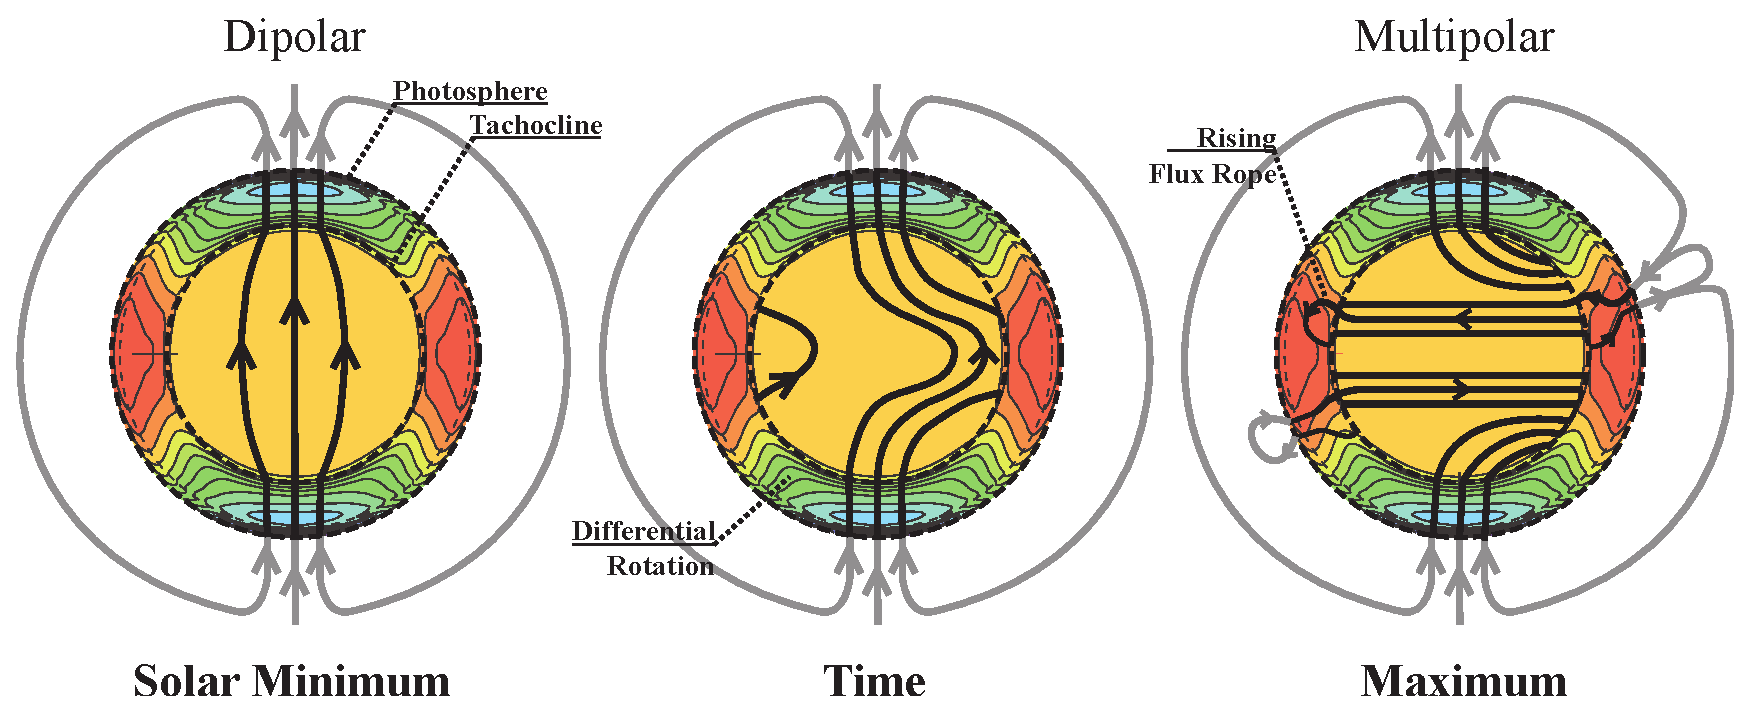
\includegraphics[width = 1.0\textwidth,clip=1]{dynamo_schem.eps}}
\caption[A summary of the magnetic solar cycle.]{A summary of the global magnetic field evolution between solar minimum and maximum. \emph{Left:} The global field is a dipole at solar minimum. \emph{Center:} Differential rotation results in dipolar field lines becoming toroidal. \emph{Bottom:} Flux ropes rise and emerge at the photosphere as sunspot groups.}
\label{fig:globalsummary}
\end{figure}

A $\sim$22\,year cycle is observed which includes two sunspot cycles. When this cycle begins at ``solar minimum", characterized by a minimum in the number of sunspots observed to emerge over time,  the global magnetic field is bipolar with magnetic north matching the spin-axis north pole. The global dipolar field lines are then displaced longitudinally and stretched into a toroidal configuration due to differential rotation, in which the rotational angular velocity of the Sun decreases with latitudinal distance from the equator. As the global bipolar field becomes toroidal, the polar magnetic field strengths decrease and a sharp increase in the number of emerging sunspots is observed. For several years during sunspot maximum, the global dipole switches polarity and the spin-axis north pole becomes magnetic south. Over the course of the next $\sim$6\,years, the frequency of sunspot emergence decreases to a new minimum and the second half of the 22~year cycle follows, similar to the first, but with a flipped global dipole. The process from solar minimum to maximum is illustrated in Figure\,\ref{fig:globalsummary}.

%By tracking many magnetic flux elements over an entire solar cycle we aim to determine the precise characteristics of this flow.
%The likely candidate for carrying magnetic flux to the poles, resulting in reversal, is the meridional flow which is observed to originate at the equator and flow in either direction, poleward. 
It is commonly understood that during the solar cycle the polar fields are reversed by the accumulation of weak magnetic flux elements at high latitudes, carried from lower latitudes \citep{Babcock:1961, Leighton:1964}. It is thought that the combination of Joy's Law, the poleward meridional flow, and supergranular diffusion allow this process to occur \citep{Mosher:1977}. Small flux concentrations are carried to the poles more swiftly (than would be due to their diffusive random walk alone) by the meridional flow. The meridional flow itself has been indirectly measured using both surface tracking methods and helioseismology techniques \citep{Hathaway:2010,Haber:2002,Zhao:2004}. Since following (leading) flux concentrations in bipoles tend to be weaker (stronger), they are more affected by flows \citep{Schrijver:1996}. Thus slightly more (less) of the flux of the following (leading) polarity will random-walk to the nearest hemispheric pole before completely decaying. The process has been studied extensively by directly observing large scale quiet-Sun magnetic fields \citep{Harvey:1992,Ulrich:2005,Schrijver:2008b} and by using surface flux transport models \citep{Leighton:1964,Wang:1989,Schrijver:2003}. These models are able to qualitatively reproduce the evolution of the distribution of photospheric magnetic fields on the Sun. 

\citet{Ulrich:2002} shows that the global dipole field reversal is driven by the bursty emergence and poleward migration of ARs over a short period of time, rather than a continuous flux emergence process. The meridional flow latitude profile has been measured using Doppler data \citep{Ulrich:2005}, surface feature tracking methods \citep{Hathaway:2010}, and helioseismology techniques \citep{Haber:2002,Zhao:2004}. Each study presents observations of a reverse of direction in the meridional flow at high latitudes at different phases in the solar cycle. \citet{Schrijver:2008b} use measurements of the dipole strength and surface flux transport modeling to conclude that this dynamic meridional flow is responsible for cycle to cycle differences in the polar field strengths.

%EQN Dipole moment/Quadrupole moment etc
The imbalance of net magnetic flux is an observational effect resulting from summing the signed magnetic flux within a limited surface area on the Sun. It is important in the analysis of the large-scale magnetic field. Hemispheric flux imbalance, the magnetic polarity imbalance between the North and South hemispheres, affects the structure of the global magnetic field. For instance, a purely dipole field results from having a single opposing polarity in each hemisphere. In reality, the Sun's field is multipolar.
%4.1-hemispheric imbalance must be open flux or faraway conection. likely not trans longitude, probably trans hemisphere
Large scale measurements of the imbalance between outward (positive) and inward (negative) directed magnetic flux from 1975-2000 have been studied by \citet{Choudhary:2002} and it is seen that hemispheric flux imbalance is a function of the solar cycle and furthermore switches sign between cycles. A clear signal is found in the northern hemisphere, but is much less clear in the southern. Upon measuring flux imbalance in individual ARs, a larger percentage imbalance is found than that determined hemispherically. It is reasoned that this indicates ARs must be balanced by long-range connections to oppositely imbalanced ARs at similar latitudes and the hemispheric imbalance is resolved by trans-equatorial connections. If ARs were balanced using trans-equatorial connections then the hemispheric imbalance could be much larger.

\begin{landscape}
\begin{figure}
\centering{\includegraphics[width = 1.2\textwidth]{hath_bfly.eps}}
\caption[The sunspot cycle over $\sim$150\,years.]{The sunspot cycle over $\sim$150\,years \citep[from][]{Hathaway:2010b}. \emph{Top}: the number of sunspots at each latitude over time. This plot exhibits the characteristic butterfly shape. \emph{Bottom}: the total number of sunspots over time. The 11-year cycle is seen to occur with a varying peak sunspot number.}
\label{fig:sunspotnum}
\end{figure}
\end{landscape}

%%%%%%%%%%%%%%%%%%%%%%%%%%%%%%%%%%%%%%%%%%%%
\subsection{Global Field Reversal}\label{intro:fieldreversal}

The large-scale configuration of the magnetic field within the convection zone is thought to transition between being poloidal and toroidal, every 11\,years \citep{Parker:1955}. The process which facilitates this reorganisation is the magnetic dynamo. Longitudinal flows drag poloidal fields into a toroidal configuration and meridional flows then help to reverse the process. The poloidal field is measured at the North and South poles of the Sun during solar minimum \citep{Harvey:2002}. The large-scale toroidal field has also been directly measured by taking advantage of line-of-sight magnetic field measurements at the solar limb \citep{Ulrich:2005}. Toroidal fields at the tachocline are stretched into thin twisted flux ropes by shearing at the interface of the rigidly rotating radiative zone and regions where the differentially rotating convection zone is moving at a different speed. Turbulent perturbations introduce instability into the flux ropes and magnetic buoyancy becomes important and causes them to rise toward the surface, as described in Section \ref{intro:aremerge}.

%FLUX TRANSPORT MODELS
The combination of these phenomena causes a reversal of the polar magnetic fields \citep{Babcock:1961,Leighton:1964}. The Babcock-Leighton process can be seen in large-scale magnetogram observations \citep{Harvey:1992} and successfully reproduced using surface flux transport models \citep{Wang:1989,Schrijver:2003}. These models imply a buildup of net magnetic flux (an imbalance of $+$ and $-$ magnetic polarities) should occur at mid to low latitudes of the same polarity as the pole in that hemisphere. At higher latitudes, flux of one polarity builds up as magnetic elements are swept poleward. Low latitude flux from opposite hemispheres eventually diffuses toward the equator and cancels or submerges. Since net flux must sum to zero globally, one should measure the same magnitude, but opposite sign, of net flux at high and low latitudes in each hemisphere. For the first time we present a quantitative comparison of the amount of imbalanced flux in the AR bands and at high latitudes (Section \ref{subsect_imbharm}).
Regardless of the vehicle for flux decay and redistribution, the total observed flux decreases but physically the net flux must be conserved due to the solenoidal constraint (Gauss' Law), as there are no magnetic monopoles ($\nabla\cdot\mathbf{B}=0$).
Locally on the Solar surface, non-zero positive (negative) net flux may exist as it may be connected to distant negative (positive) flux concentrations, or may be quasi-open (connected to the solar wind) and balanced by other quasi-open negative (positive) flux concentrations on the solar surface.

%BUTTERFLY DIAGRAM
Latitudinal observations of net flux over time show that while the active region belt progresses from high to low latitudes, net unipolar flux is observed to be transported poleward, as observed in magnetic butterfly diagrams \citep{Harvey:1992}. \citet{Choudhary:2002} investigate large-scale flux imbalances finding that the signed flux imbalance between the North and South hemispheres is a function of the solar cycle and furthermore switches sign between cycles. \citet{zharkov:2006} study flux imbalance in individual sunspot groups statistically for a portion of solar cycle 23. Opposite imbalances in each hemisphere are found that reverse at the solar minimum. \citet{Zharkov:2008} state that a phase relation exists between active region flux imbalances and the background high-latitude magnetic field. These results support the Babcock-Leighton model.

%EQN Dipole moment/Quadrupole moment etc
The properties of detected ARs, such as flux imbalance, affect the solar magnetic structure locally, while on a global scale, hemispheric flux imbalance affects the structure of the solar magnetic field. For instance, a purely dipole configuration results from having a single opposing polarity in each hemisphere. 
\citet{mordvinov:2007} determines a relationship between the IMF and global field harmonic modes-- especially the $[l=2,m=0]$ mode.
Generally, the global field is multipolar and we can describe its structure extending into the solar atmosphere using the superposition of spherical harmonics, with a potential field source surface (PFSS) model. 

Some studies focus on periodicities in the harmonic coefficients over multiple solar cycles finding separate frequencies in axisymmetric and non-axisymmetric modes \citep{stenflo:1986, stenflo:1988, knaack:2005}.
It has been determined that to accurately predict the magnetic field at Earth, the properties of low latitude magnetic features on the Sun must be taken into account \citep{schussler:2006, wang:2003a, Schrijver:2003}. The distribution of open flux and the global field configuration determine the shape of the heliospheric field and thus can affect the space weather environment at Earth.
Taking these findings into account, we seek to better understand the evolution of the global solar magnetic field in the context of a full 11\,year activity cycle (half of a magnetic cycle) by characterizing spatio-temporal distributions of magnetic feature properties.

%%%%%%%%%%%%%%%%%%%%%%%%%%%%%%%%%%%%%%%%%%%%
\subsection{Active Sunspot Groups}\label{intro:flareactreg}

%Sunspot groups are formed by the convective action of sub-surface fluid motions pushing magnetic flux tubes through the Sun's surface, the photosphere. Turbulent photospheric and sub-photospheric motions jostle around these flux tubes and, when the conditions are right, the sunspot group produces a flare \citep{Conlon:2010a}. 
Sunspots are formed beneath the solar surface and emerge through the photosphere and into the corona. Turbulent photospheric and sub-photospheric motions jostle around the constituent flux tubes of the flux ropes that form sunspots, possibly resulting in destabilisation that leads to a flare \citep{Conlon:2010a}. Other phenomena, such as shearing and helicity injection, may build up stress in an AR leading to strong electric currents that correlate with flaring \citep{Schrijver:2005,Schrijver:2007}. 
Currently the exact conditions that are necessary for or lead to flaring are not known. This is partly due to limitations in our observational capabilities. Only the magnetic fields at the foot points of sunspot groups can be imaged, while flares actually occur some distance above the sunspot in the solar atmosphere. Flaring sunspot groups tend to be big and ugly (and thus bad). The largest eruptions and flares are released by large but compact sunspot groups with complicated magnetic configurations. In this section we will refer to active magnetic structures, including sunspot groups, as ``active regions" to include the entire system (surrounding magnetic flux elements and loop structures in the corona) connected to a flare.

\begin{figure}[!t]
\centerline{\includegraphics[width = 0.7\textwidth,clip=1]{McIntosh_1990_class.eps}}
\caption[The McIntosh sunspot group classification system.]{The McIntosh sunspot group classification system \citep[from][]{McIntosh:1990} The left column depends on the presence of spot penumbrae and group length. The middle column indicates features of the largest spot's penumbra. The right column is determined by the amount of spot coverage between the leading and trailing edges of the group.}
\label{fig:mcintoshclass}
\end{figure}

Several classifications of active regions were designed to describe alternatively white-light and magnetogram observations of sunspot groups. The most common, McIntosh classification (Figure~\ref{fig:mcintoshclass}), is an expansion of the Zurich system. It describes the number and development of sunspots within a group, including properties of umbrae and \glspl{penumbra}. \cite{McIntosh:1990} finds that the scheme is adept at indicating the relative flare productivity of a given class. 

The Hale classification system classifies the distribution of polarities in the active region, as described by Table~\ref{fig:haleclass}. This system has been expanded to include the $\delta$-class, which is given when two polarities are present within a single sunspot \gls{penumbra} \citep{Kunzel:1960}. The $\alpha$ indicates only one polarity of spot is visible, with p (f) meaning that any spots precede (follow) the magnetic field distribution. The $\beta$ indicates both spot polarities of spot are visible with p and f indicating which spot is larger. The $\gamma$ indicates spots of one polarity are on both sides of one or more spots of opposite polarity. Sunspot groups denoted as $\delta$-class are shown to produce the most significant flares \citep{sammis:2000}. These classification schemes are well correlated to quantitative descriptions of active region complexity \citep{ireland:2008}. 

%\begin{figure}[!t]
%%\centerline{\includegraphics[width = 0.5\textwidth]{images/hale_class.pdf}}
%\caption{...}
%\label{fig:haleclass}
%\end{figure}
\begin{table}[!t]
\caption[The possible sunspot group classifications using the Hale scheme.]{The possible sunspot group classifications using the Hale scheme \citep{Hale:1919} with the appended $\delta$-class \citep{Kunzel:1960}. The ``p" (``f") denote whether the strongest spot is preceding (following).}
\centering{
\begin{tabular}{lll}
\hline \hline
Unipolar & Multipolar & Mixed \\
\hline
$\alpha$ & $\beta$ & $\beta\delta$ \\
$\alpha$p & $\beta$p & $\beta\gamma\delta$ \\
$\alpha$f & $\beta$f & \\
& $\beta\gamma$ & \\
\hline
\end{tabular}
}
\label{fig:haleclass}
\end{table}

%REORGANISE THESE PARAGRAPHS INTO property types
Classification has been shown to be useful for grouping active regions by their expected flare productivity. The quantification of active region properties allows a physical comparison and deeper understanding of the actual causes flaring. Complexity, often quantified by fractal index \citep{mcateer:2005b,Conlon:2008,Conlon:2010a} and scale-power distributions \citep{Abramenko:2005,Hewett:2008} is shown to be correlated with flare productivity. However, recent work has shown that fractal dimension is not a good flare predictor \citep{georgoulis:2012}. 
The presence of shear and helicity injection are shown to initiate flaring within active regions \citep{Schrijver:2008a}.
Strong polarity separation lines with large gradients and large field magnitudes on either side are known to be one of the best indicators of flaring \citep{Schrijver:2007}.

Generally active regions emerge up to a certain size while their non-potential characteristics (such as polarity separation line strength) continue to evolve. Upon reaching a state of maximum complexity, active regions are observed to produce the most significant flares. The relationship between flux and the sum of magnetic gradients along a polarity separation line (\gls{wlsg}) is shown to be a power law \citep{Falconer:2009}. 

Various statistical methods have been used in conjunction with an assortment of physical properties to forecast flares. %Much work has been done using these properties to forecast flares (Section \ref{intro:flareforecast}).
Current forecasting systems are limited \citep{Messerotti:2009} and often generate incorrect predictions. The inaccuracy of forecasting systems may be very costly. Depending on the application, false alarm forecasts may result in lost revenue during satellite shut-downs, diverting trans-polar flights, delayed spacecraft launches. On the other hand, missed flares could result in damage to sensitive space-born instruments, such as those on communications, scientific, or military satellites, or the endangerment of pilots on transpolar flights and astronauts on space-walk \citep{national2008Severe}. In 1989 a solar storm caused disruptions to power grids in Quebec, the northeastern United States, and areas of Sweden causing blackouts for hours. Recently, communications with the civilian Galaxy 15 satellite were compromised in April 2010, and the spacecraft was unable to respond to commands from the ground for months. As our society and military become increasingly technologically advanced, we become more directly affected by solar activity.

Past work on predicting the occurrence of flares in sunspot groups has focused on determining a set of sunspot group properties important for flaring \citep{Gallagher:2002}. This requires a large set of characterized sunspot group detections, which is used to train a prediction system. Automated detection and characterization systems, such as the SolarMonitor Active Region Tracker \citep[SMART;][]{higgins:2011} developed by our team, are useful for this task and often focus on characterizing magnetic field properties. Using these detection methods, modules may be applied to determine various properties: size; magnetic flux; polarity separation line length; magnetic energy; magnetic connectivity. The sunspot group detections are then associated with a flare catalog and correlations are determined for specific properties and various prediction time windows and latencies.

There have been many studies attempting to find the most significant sunspot group properties for predicting flares. \cite{Leka:2003a,Leka:2003b,Leka:2007} and \cite{Barnes:2006} test a large number of vector magnetic properties (e.g., moments of the vector magnetic field, magnetic shear, and current helicity) in various combinations and find that characterizing a sunspot group at one point in time has limited bearing on whether it will flare in the future. 

More recent work, such as \cite{Colak:2009} and \cite{Ahmed:2011} rely on machine learning algorithms using a database of sunspot group properties and knowledge of flare occurrence as input. Much more accurate flare prediction results are achieved, while much fewer properties are investigated than previous studies.  \cite{Colak:2009} rely on automated McIntosh sunspot classifications as a property, generated using another machine learning algorithm. Alternatively, \cite{Ahmed:2011} use the line-of-sight magnetic properties defined in \cite{higgins:2011} and listed in Tables\,\ref{tablemagprop} and \ref{tablehighorder}. The descriptors with the most predictive power were found to be \gls{PSL} length ($L_{PSL}$), strong gradient \gls{PSL} length ($L_{sg}$), maximum horizontal magnetic field gradient ($\nabla( B)_{max}$), the sum of the gradient along $L_{sg}$ ($WL_{sg}$), the sum of the gradient along $L_{PSL}$ ($WL^*_{sg}$), and the total magnetic flux near the \gls{PSL} ($R^*$).

Using a completely different approach, \cite{Wheatland:2005} achieves good results predicting flares on the assumption that if a flare has occurred, more will occur. This shows that the history of activity of a sunspot group is a significant predictor. For the purposes of reliable operational forecasting, all existing systems are still limited, as their use results in substantial numbers of false alarms and missed flares. 

Most studies use point-in-time detections of sunspot groups to predict flares. \cite{Mason:2010} are an exception, and show promise in predicting flares using previous changes in magnetic properties. %Figure 2 shows the magnetic evolution of a tracked sunspot group as compared with its flare productivity. 
The concept of relating sunspot group dynamics and evolution has not been extensively explored.

%\begin{table}
%\caption{The observation-prediction contingency table, or affectionately as the ``confusagram". }
%\centering{
%\begin{tabular}{c|c|c}
%\hline \hline
%& Observed & Not Observed \\
%\hline
%'Yes' Forecast & TP & FP \\
%\hline
%'No' Forecast & FN & TN
%\end{tabular}
%}
%\label{table:conttable}
%\end{table}

%To compare the effectiveness of these forecasting systems several accuracy and skill scores have been appropriated from the climate sciences. These are calculated using a contingency table, as shown in Table~\ref{table:conttable}. Flare truth indicates whether or not a flare actually occurs, while forecast indicates whether one was predicted to occur. The elements of the table are true positives (TP) when a flare has occurred and was predicted, false negatives (FN) when a flare has occurred but was not predicted, true negatives (TN) when no flare has occurred and none was predicted, and false positives (FP) when no flare has occurred but one was predicted to occur. 
%Common forecast validation measures are, 
%\begin{eqnarray}
%accuracy &=& \\
%probability of detection &=& \\
%false alarm rate &=& \\
%heidke skill score &=& \\
%true skill statistic &=& \\
%\end{eqnarray}

%REF wilcox 1973? balch?

%%%%%%%%%%%%%%%%%%%%%%%%%%%%%%%%%%%%%%%%%%%%
\section{Solar Eruptions}\label{intro:solerupt}
%%%%%%%%%%%%%%%%%%%%%%%%%%%%%%%%%%%%%%%%%%%%

Solar eruptive activity is associated with large complex sunspot groups. The solar activity cycle is mainly observed by monitoring the number of sunspots on disk (sunspot number). On $\sim$year timescales the number of eruptive events observed is well correlated with the sunspot number. Each eruption is different and there are a wide variety of phenomena that are generally associated with them. To present a common scenario: often, as a sunspot group evolves, material can cool and collect in a ``channel", suspended above by the magnetic loop structure along a sheared \gls{PSL}. This material is called a filament or prominence depending whether it is observed from above or side-on. The shear and twist in the system introduces magnetic stresses. At some point an instability occurs and the fields are thought to rapidly reorganise to a lower energy state. Theoretically, this reorganisation releases part of the stored magnetic energy as radiation and non-thermal particle acceleration \citep{Fletcher:2011}. This conversion and release of energy is called a flare. The converted magnetic energy is considered to be part of the ``non-potential" portion of the magnetic energy in the system, as discussed in Chapter~\ref{chapter:theory}. Often this is accompanied by the release and acceleration of matter called a \gls{CME} which carries another large portion of the energy. The kinetic \gls{CME} energy has been shown to be greater, but of the same order of magnitude as the radiative flare energy \citep{Emslie:2004}. The accelerated matter generally includes filament material forming the ``core" and an overarching twisted magnetic loop structure called a flux rope forming the ``front" of the \gls{CME}. 

\begin{figure}[!t]
\centerline{\includegraphics[width = 0.7\textwidth,clip=1]{1_introduction/figures/flare_phases.eps}}
\caption[The progression of a typical solar flare.]{The progression of a typical solar flare \citep[from][]{Qiu:2009}. \emph{Top:} the impulsive phase is characterised by a rapid burst of hard X-rays (HXT), followed by the gradual decay of soft X-rays (GOES). \emph{Bottom left:} The contours indicate the location of HXR emission. \emph{Bottom right:} During the course of the flare, the foot points move apart, as indicated by the colored marks.}
\label{fig:flarephase}
\end{figure}

Solar flares are among the most energetic events occurring in the solar system, influencing a panorama of physical systems: from the solar surface and atmosphere, through the heliosphere, and into geo-space. Flares, along with coronal mass ejections, are a major contributor to space weather:  the interaction of magnetic fields and particles accelerated on or near the Sun with the Earth's magnetosphere and upper atmosphere. Although significant progress has been made in understanding the fundamental physics of flares, their accurate forecasting remains impossible.

Flares occur in volumes of the atmospheric plasma above sunspot groups with increased emission at temperatures of 1\,000\,000\,K or more. There are many flare cartoons which mainly rely on the release of magnetic energy through reconnection\footnote{See: \url{http://solarmuri.ssl.berkeley.edu/\~hhudson/cartoons/}.}. 
%During reconnection, large currents lead to heating which is observed at the tops of coronal loops. Additionally, particles stream down the loop legs, resulting in heating at their foot points in the chromosphere. 
%If the process is attributed to reconnection a ``breakage" of field lines occurs and acceleration of a plasmoid. This plasmoid can become a \gls{CME}. Often a filament lies over the flaring structure and subsequently lifts off, becoming the core of a \gls{CME}. 
It is thought that magnetic reconnection occurs at strong current sheets where magnetic fields are oppositely aligned, causing particle acceleration. Their occurrence tends to be along polarity separation lines \citep{Schrijver:2007}. High-energy particles stream down the legs of the reconnecting structure, impacting the chromosphere, and producing \gls{EUV} and X-ray radiation. High energy X-ray, or \gls{HXR}, emission is concentrated at the foot points and the apex of the structure near the reconnection region. Lower energy, or \gls{SXR}, emission is focused in different regions depending on the phase of the flare evolution, but is generally more widely distributed over the loop structure.

\begin{figure}[!t]
\centerline{\includegraphics[width = 0.7\textwidth,clip=1]{1_introduction/figures/aschwan_flare_freq.eps}}
\caption[The frequency distribution of flare magnitudes measured in various studies.]{The frequency distribution of flare magnitudes measured in various studies \citep[from][]{Aschwanden:2011}.}
\label{fig:flaredist}
\end{figure}

There are several stages in the evolution of a flare: the pre-flare, impulsive, and gradual phases \citep{Fletcher:2011}. The behaviour of emission at different wavelengths and the motions of the flare foot points is shown in Figure~\ref{fig:flarephase}. In the pre-flare phase, heating occurs that signals the oncoming flare. This often takes the form of a filament activation that is observed as a brightening of filament material in H-$\alpha$ observations. During the impulsive phase, rapid brightenings in \glspl{HXR} and radio (type III bursts) are observed. The main brightening in \gls{SXR} occurs more slowly and its peak divides the impulsive and gradual phases. During the initial \gls{SXR} brightening and peak, the shape of the time profile of \gls{HXR} emission generally follows the time derivative of the \gls{SXR} emission. This is called the Neupert effect and is thought to occur because the cooling timescale of coronal \gls{SXR} emitting plasma is longer than that of the chromospheric heating mechanism. Electrons accelerated during the flare cause non-thermal \gls{HXR} emission and chromospheric ``evaporation" that heats the corona above, resulting in thermal \gls{SXR} emission. This effect was first noted by \cite{Neupert:1968} by comparing X-ray and microwave observations.

\begin{table}
\caption[The GOES flare classification scheme.]{The GOES flare classification scheme, where peak fluxes are integrated over the 1-8\,\AA\ bandpass.}
\label{tab:gclass}
\centering{
\begin{tabular}{lc}
\hline \hline
Class & Peak Flux [W\,m$^{-2}$] \\
\hline
X10 & $10^{-3}$ \\
X & $10^{-4}$ \\
M & $10^{-5}$ \\
C & $10^{-6}$ \\
B & $10^{-7}$ \\
A & $10^{-8}$ \\
\hline
\end{tabular}
}
\end{table}

Large flares release around $10^{32}$\,erg of energy through radiation. They are often characterised by the magnitude of their peak emission in \glspl{SXR} using a 1-8\,\AA\ bandwidth. This classification system is a base-ten magnitude system called the GOES Class after the instrument used to define it and is summarised by Table~\ref{tab:gclass}. Each higher class of flare exhibits peak SXR emission ten times greater than the last. With in a single class, flares are usually ordered by the first two significant digits of their flux. For example, a flare with a peak flux of $4.5\times10^{-5}$\,W\,m$^{-2}$ would be given a classification of M4.5. The frequency flare occurrence with increasing magnitude follows a decreasing power law. A slope between -1.5 and -2.5 is measured in various studies \citep[see Figure~\ref{fig:flarephase};][]{Aschwanden:2011}. 
Also, the distribution of waiting times between flares over long time-scales has been shown to be a power law over time-scales greater than a few hours, pointing to an avalanche model \citep{Lu:1993}, but is exponential when considering the statistics over multiple solar cycles, indicating flaring is a random Poisson process \citep{Wheatland:2000}. Individual active regions exhibit an exponential distribution of flaring rates \citep{Wheatland:2001} and it is well known that the best predictor for a flare to occur in the future is that a flare has occurred in the past \citep{Wheatland:2005}.

%%%%%%%%%%%%%%%%%%%%%%%%%%%%%%%%%%%%%%%%%%%%
\section{Thesis Aims}\label{intro:aims}
%%%%%%%%%%%%%%%%%%%%%%%%%%%%%%%%%%%%%%%%%%%%

Very few sunspot-related phenomena are well understood. It is only superficially known how the large-scale plasma circulation and the decay and dispersion of sunspot magnetic fields are connected to the reversal of the global magnetic field. Above the photosphere, the magnetic field strength and structure can only be roughly estimated, and below the photophere neither is known to any certainty. Additionally, predicting the strength of the next solar cycle, the frequency of sunspot emergence, and the occurrence of flares with the accuracy required by the operational community is not possible. 

The aim of this thesis is to better understand the evolution of individual sunspot groups and the global magnetic field. The study aims to address three questions in a series of studies:
\begin{itemize}
\item \emph{What are the conditions in sunspot groups that result in solar flares?} The relationship between flaring and sunspot group property dynamics is investigated. Property distributions associated with different flare magnitudes are compared. The properties of sunspot groups over the solar cycle are compared to global flare productivity. 
\item \emph{What mechanisms determine the configuration of the global magnetic field and how does this relate to the solar dynamo?} The distribution of magnetic features affects the global magnetic field of the Sun. A comparison between the properties of sunspot groups and the global field configuration over solar cycle 23 is presented. 
\item \emph{What mechanisms govern the evolution and decay of sunspot groups?} A mechanism for the decay of sunsot groups is investigated by comparing a large-scale observation of magnetic field dispersion to a simulation. 
\end{itemize}
To allow a large-scale study of the solar magnetic field, a combination of image processing techniques is used to automatically detect, characterise, and track sunspot groups over time.

The remainder of this thesis is organised as follows.
The theory describing magnetic fields in a plasma is presented in Chapter~\ref{chapter:theory}. 
The magnetic field observations and other data used in the investigations are described (see Chapter~\ref{chapter:data}). 
The methods for automatically detecting and characterising sunspot groups are described in \ref{chapter:method_SMART}. 
Three scientific studies of the solar magnetic field follow in Chapters~\ref{chapter:results_activity}, \ref{chapter:results_global}, and \ref{chapter:results_diffusion}.
Finally, the main results and conclusions of the studies, including prospects for future work, are summarised in Chapter~\ref{chapter:discussion}.